\sectionorchapter*{Introduction}
\eggorcadmo{}{\label{introduction}\addcontentsline{toc}{chapter}{\nameref{introduction}}}
In the study of plane embeddings of planar graphs, also known as plane graphs,
embeddings with non-crossing straight edges (called crossing-free geometric graphs) are of particular
interest.
For instance, it is known \cite{LeeuwenSchoone1981} that any optimal solution to the travelling salesman problem in the
Euclidean plane has non-crossing straight edges.
In 1935, K.~Wagner proved \cite{Wagner1936} that any planar graph has such an
embedding.

\begin{sloppypar}
A natural enumerative question is then, given a vertex set of $n$ points in the Euclidean plane,
to bound the number of plane graphs of a certain sort (cycles, matchings, \etc.) which can be
drawn with non-crossing straight edges.
For spanning cycles, the question was introduced by M.~Newborn and W.~O.~J.~Moser in 1976 \cite{NewbornMoser1980},
and a super-exponential upper bound was given.
In 1980, M.~Ajtai, V.~Chvátal, M.~Newborn, and E.~Szemerédi \cite{AjtaiChvatalNewbornSzemeredi1982}
proved that there are only exponentially many crossing-free geometric graphs on a given point set.
\end{sloppypar}

Exponential bounds for various sorts of graphs were then improved, in particular for triangulations---the
maximal crossing-free geometric graphs. One of the interesting features of triangulations is that finding a bound for
them yields a bound for the overall number of crossing-free geometric graphs \cite{AjtaiChvatalNewbornSzemeredi1982}.
In addition, bounds on the number of triangulations
are of interest in geometric modeling, see for instance \cite{Smith1989}.

Some special configurations of points are better understood; in particular, for point sets in convex position,
the numbers of crossing-free perfect matchings, triangulations, and spanning cycles are known. In fact, the study
of point sets in convex position vastly predates the general problem, with the number of triangulations given by
Euler in 1751 \cite{Euler1751}.

For perfect matchings, an optimal lower bound of $\CatalanNumber {\frac n 2}$ (where $\CatalanNumber k$ is the $k$th Catalan
number, see section~\ref{TriangulationsAndCatalan}) was obtained as early as 1995 by A.~García,
M.~Noy, and J.~Tejel \cite{GarciaNoyTejel2000}; upper bounds have been harder to come by, with the best one
yet being asymptotically $10.05^n$, given by M.~Sharir and E.~Welzl in 2005 \cite{SharirWelzl2006}
In that same work, an upper bound of $5.83^n$ is given for the number of crossing-free perfect matchings on a
point set whose points are designated as left or right endpoints; moreover, an upper bound of $4^n$ is given
when all the left endpoints are to the left of the right endpoints (matchings across a line).

In this thesis, 
we start by giving an overview of some of the existing results, in particular a way
to classify arrangements of designated left and right endpoints,
and we restate the proof of the bound for matchings across a line by M.~Sharir and E.~Welzl
(\sectionorchapterword~\ref{sectionBackground}).
We then study in detail the inequalities in that bound and the objects it actually counts,
yielding criteria that will allow us to tighten the bound in specific cases (\sectionorchapterword~\ref{sectionOvercounting}).
Using these criteria, we give a bound for
matchings across a line that depends on the number of points in the interior of the convex hull
(\sectionorchapterword~\ref{sectionHighlyConvex}).
We then give new bounds on the number of crossing-free perfect matchings on a point set with designated left and
right endpoints for a specific family of left-to-right orderings of the left and right endpoints
(\sectionorchapterword~\ref{sectionThreeChanges}), namely orderings where, from left to right, the endpoint designation
changes three times (thus left endpoints, then right endpoints, left endpoints, and finally right endpoints).
\sectionorchapter{Background}
\label{sectionBackground}
We first give some definitions, as well as existing proofs whose ideas we will use to derive our results.
\subsectionorsection{Geometric graphs}
\begin{definition}[geometric graph]
Given a set of points $\pointset P$ in the Euclidean plane $\R^2$,
a \emph{geometric graph} is a collection of straight line segments (edges)
whose endpoints are elements of $\pointset P$.
\end{definition}
A geometric graph can be described as a simple graph (in the combinatorial sense)
on the vertices $\pointset P$, where the edge $\set{p,q}$ corresponds to the segment joining
$p$ and $q$.
\begin{sloppypar}
\begin{definition}[crossing-free]
A geometric graph is \emph{crossing-free} if no two edges share points other than
their endpoints; it is called \emph{crossing} otherwise.
\end{definition}
Note that being crossing-free implies that the corresponding simple graph is planar, and that the
geometric graph is a plane embedding.
\begin{definition}[triangulation]
A \emph{triangulation} is a maximal crossing-free geometric graph, that is, a
geometric graph such that for all $p$ and $q$ in $\pointset P$ that are not joined by a
segment, adding the segment joining $p$ and $q$ would result in a crossing
geometric graph.
\end{definition}
Note that the faces (in the sense of plane graphs) formed by a triangulation are
all triangles, with the possible exception of the outer face (thus this definition
is \emph{not} equivalent to that of a triangulation of the $2$-sphere).
\end{sloppypar}

Since a geometric graph corresponds to a simple graph on the underlying point set,
we can also look at geometric graphs that belong to special classes of simple graphs.
As we will only be focusing on geometric graphs, we simply call
\emph{perfect matching}
a geometric graph which corresponds to a perfect matching in the combinatorial sense.

As outlined in the introduction, we are interested in statements regarding the number
of geometric graphs, possibly restricted to a certain type, on a given point set.
Evidently, that number would depend on the choice of the point set $\pointset P$, so instead we seek
bounds on that number depending on the cardinality $\Cardinality {\pointset P}$, and possibly
restricting $\pointset P$ so that it satisfies certain properties.

An important property that $\pointset P$ can have is general position. We say that 
a point set in the plane is \emph{in general position} if no three points are collinear.
In this thesis we will only study point sets in general position.

In general, if $g\of {\pointset P}$ is the number of geometric graphs of a certain sort on the point
set $\pointset P$, we will look for lower bounds $l$ and upper bounds $u$ of the form\[
\forall n\in \N, \forall \pointset P \text{ such that } \Cardinality {\pointset P} = n,
l \of n \leq g \of {\pointset P} \leq u \of n \text,\]
where $\pointset P$ runs over all point sets that satisfy the relevant properties.

\subsectionorsection{Asymptotics}
In addition, we will want asymptotics on such bounds $l$ and $u$, to compare them with
existing results. Since the bounds are often exponential, we tend to ignore polynomial
factors. We will thus write that\[
u \of n \preccurlyeq_n f \of n
\]
if for some polynomial $\gP$, $\forall n\in \N, u\of n \leq \gP\of n f \of n$.

In some cases, we may be interested in classes of functions $g_z\of{\pointset P}$
which depend on some parameter $z\in\gW_n$, where $\gW_n$ is a set of arbitrary objects.
For instance, $g_z$ could count crossing-free graphs on $\pointset P$ that contain an independent set
of size $z\in [n]$.
In this thesis, we will often use classes $g_z$ with $z$ being the left-to-right ordering
of designated left and right endpoints---this will be formalized in section~\ref{bracketExpressions}.

When giving exponential bounds in $n$ for these parameterized classes of graphs, we will want to keep
track of any dependence on $z$. We will write that\[
u \of {n,z} \preccurlyeq_n f \of {n,z} \text{ \emph{uniformly in $z\in\gW_n$}}\]
if for some polynomial $\gP$ (that does not depend on $z$),
\[\forall n\in \N,\forall z \in \gW_n, u\of {n,z} \leq \gP\of n f \of {n,z}\text.\]
If $f \of {n,z}$ admits a supremum $F \of {n}$ in $z\in\gW_n$ for all $n$, this implies
that $u\of {n,z} \leq \gP\of n F \of{n}$, giving an upper bound truly independent of $z$.
It also makes it possible to get a bound by summation of $f \of {n,z}$ over $z\in\gW_n$.

Observe that these bounds up to a polynomial are related to $\BigO$ notation when the upper bound
is exponential; specifically, for $\gz>1$,
\[u \of n \preccurlyeq_n \gz^n \Implies \forall\gce>0, u\of n\in\BigO\of{\pa{\gz+\gce}^n}\text.\]
Moreover, we can bound a product by the product of the bounds for its factors. Specifically,
for positive $f_1$ and $f_2$, if
$u_1\of{a,z}\preccurlyeq_a f_1\of{a,z}$ and
$u_2\of{b,z}\preccurlyeq_b f_2\of{b,z}$,
both uniformly in $z$, we have\[
u_1\of{a,z}u_2\of{b,z}\preccurlyeq_{m} f_1\of{a,z}f_2\of{m-a,z}
\]
uniformly in $b\in\intclos 0 m$ and in $z$. Indeed, if $u_i\of{a,z}\leq \gP_i\of{a} f_i\of{a,z}$,
where without loss of generality the coefficients of $\gP_i$ are positive, we get
\begin{align*}u_1\of{a,z}u_2\of{a,z}
&\leq \gP_1\of{a}\gP_2\of{b} f_1\of{a,z}f_2\of{b,z}\\
&\leq \gP_1\of{a+b}\gP_2\of{a+b} f_1\of{a,z}f_2\of{b,z}\text.\end{align*}
\subsectionorsection{A remark on the asymptotics of the binomial coefficient}
Unsurprisingly, binomial coefficients will be involved in the bounds, so we now give a uniform exponential
upper bound for them.
It can be shown, by writing the logarithm of the factorial as a sum of logarithms,
and then bounding that sum by integrals, that\[
\forall k\in \Positives, \E \pa{\frac{k}{\E}}^k \leq \Factorial k \leq k \E \pa{\frac{k}{\E}}^k\text,
\]
where $\Positives\DefineAs\N\setminus\set{0}$.
It follows that\begin{align*}
\forall k\in \Positives, \forall \gh\in\intopen 0 1, \binom{k}{\gh k} &\leq
\frac{k \E \pa{\frac{k}{\E}}^k}{\E \pa{\frac{\gh k}{\E}}^{\gh k} \E \pa{\frac{\pa{1-\gh} k}{\E}}^{\pa{1-\gh}k}}\\
&=\frac{k}{\E} \frac{k^k}{\pa{\gh k}^{\gh k}\pa{\pa{1-\gh} k}^{\pa{1-\gh} k}} \\
&=\frac{k}{\E} \pa{\frac{1}{\gh^\gh\pa{1-\gh}^{1-\gh}}}^k \\
&=\frac{k}{\E} \pa{\frac{\pa{1-\gh}^{\gh-1}}{\gh^\gh}}^k\text,
\end{align*}
so that, since $\forall k\in \N, \binom k 0 = \binom k k = 1$, we have
\begin{equation}
\binom k {\gh k} \preccurlyeq_k \pa{\frac{\pa{1-\gh}^{\gh-1}}{\gh^\gh}}^k \text{ uniformly in $\gh\in\intclos 0 1$.}
\end{equation}
\subsectionorsection{Triangulations of convex point sets and the Catalan numbers}\label{TriangulationsAndCatalan}
A set of points is said to be \emph{in convex position} if it is in general position and
all points are in the boundary of its convex hull.

For points in convex position, the numbers of triangulations and perfect matchings are known.
The following recurrence, given by J.~A.~Segner in 1758 \cite{Segner1758}, defines the \emph{Catalan numbers}.
\begin{theorem}[Segner]
Let $\CatalanNumber n$ be the number of triangulations of a set of $n+2$ points in convex position.
Then $\CatalanNumber 0 = 1$, and for $n>0$, \begin{equation}
\CatalanNumber n = \sum {i=0}[n-1] \CatalanNumber i \CatalanNumber {n-i-1}\text. \label{CatalanRecurrence}
\end{equation}
\begin{proof}
Consider a set of $n+2$ points in convex position.
For $n=0$ the result is trivial, the only triangulation is an edge.

Let $n > 0$, and number the points along the boundary of the convex hull, from $0$ to $n+1$,
see figure~\ref{figSegnerRecurrence}.
The edge $e$ joining points $n+1$ and $n$ is in the boundary of the convex hull, and thus must
be in any triangulation, since no other edge can cross it. Let $i$ be the index of the third point of the
triangle containing edge $e$, which may be any of the others, from $0$ to $n-1$.

Then, restricting the triangulation to the $i+2$ points $\set{0,\dotsc,i,n+1}$ yields a triangulation
of those points.
Similarly, restricting the triangulation of the whole point set to points $i$ through $n$ yields a triangulation of
$n-i+1$ points. It follows that $\CatalanNumber n \leq \sum {i=0}[n-1] \CatalanNumber i \CatalanNumber {n-i-1}$.

Moreover, given a triangulation of $\set{0,\dotsc,i,n+1}$ and a triangulation of $\set{i,\dotsc, n}$,
adding the edge $e$ forms a triangulation of the whole point set, proving equality.
\end{proof}
\end{theorem}
\marginfig[Segner's recurrence.\label{figSegnerRecurrence}]{
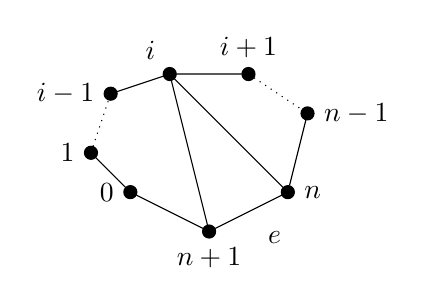
\begin{tikzpicture}[scale=0.5]
\tikzstyle{dot}=[draw,shape=circle,fill=black,scale=0.5]
\node[dot,label=left:$0$] at (1,1) (p0) {};
\node[dot,label=left:$1$] at (0,2) (p1) {};
\node[dot,label=left:$i-1$] at (0.5,3.5) (piminus1) {};
\node[dot,label=above left:$i$] at (2,4) (pi) {};
\node[dot,label=above:$i+1$] at (4,4) (piplus1) {};
\node[dot,label=right:$n-1$] at (5.5,3) (pnminus1) {};
\node[dot,label=right:$n$] at (5,1) (pn) {};
\node[dot,label=below:$n+1$] at (3,0) (pnplus1) {};
\draw (pnminus1) -- (pn);
\draw (pnplus1) -- (p0) -- (p1);
\draw (pn) -- (pnplus1) node [midway, label=below right:$e$] {};
\draw (piminus1) -- (pi) -- (piplus1);
\draw[dotted] (p1) -- (piminus1);
\draw[dotted] (piplus1) -- (pnminus1);
\draw (pnplus1) -- (pi) -- (pn);
\end{tikzpicture}}
An explicit expression for $\CatalanNumber n$ was given earlier by Euler \cite{Euler1751}, along
with the generating function.
A convenient form is\begin{equation}
\CatalanNumber n = \frac{1}{n+1} \binom {2n} {n}\text,
\end{equation}
yielding asymptotically
\begin{equation}
\CatalanNumber n \sim \frac{4^n}{n^{\frac{3}{2}}\sqrt{\Pi}} \preccurlyeq_n 4^n\text.
\end{equation}

\subsectionorsection{Crossing-free perfect matchings}
\label{PerfectMatchingsIntro}
We will call $\PM_{\pointset P}$ the set of perfect matchings on the point set $\pointset P$,
and $\CFPM_{\pointset P}$ the set
of crossing-free perfect matchings on the point set $\pointset P$.
When discussing perfect matchings, we will denote the unique edge incident to point $p$ by
$e_p$.
\marginfig[Partitioning a convex point set to construct a crossing-free
perfect matching.\label{figConvexPerfectMatching}]{
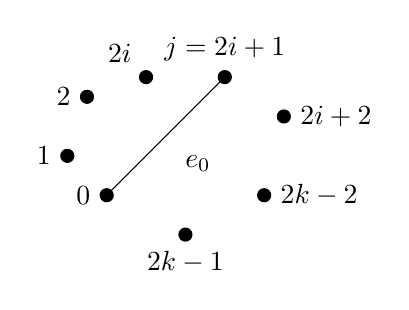
\begin{tikzpicture}[scale=0.5]
\tikzstyle{dot}=[draw,shape=circle,fill=black,scale=0.5]
\node[dot,label=left:$0$] at (1,1) (p0) {};
\node[dot,label=left:$1$] at (0,2) (p1) {};
\node[dot,label=left:$2$] at (0.5,3.5) (p2) {};
\node[dot,label=above left:$2i$] at (2,4) (p2i) {};
\node[dot,label=above:${j=2i+1}$] at (4,4) (p2iplus1) {};
\node[dot,label=right:$2i+2$] at (5.5,3) (p2iplus2) {};
\node[dot,label=right:$2k-2$] at (5,1) (p2nminus2) {};
\node[dot,label=below:$2k-1$] at (3,0) (p2nminus1) {};
\draw (p0) -- (p2iplus1) node [midway, label=below right:$e_0$] {};
\end{tikzpicture}}

If $\pointset P$ is a set of $n=2k$ points in convex position,
it was shown\footnote{In fact, Errera counts the number of figures that can be formed in the upper half-plane by $k$
non-intersecting
semicircles with their centres on the boundary. Since these are geodesics of the hyperbolic plane in the Poincaré
half-plane model, switching to the Beltrami--Klein model turns the half-plane into the unit disk, and the semicircles
into chords, so that the problem becomes that of crossing-free perfect matchings in convex position.}
by A.~Errera in 1930 \cite{Errera1931} that\[\Cardinality{\CFPM_{\pointset P}}=\CatalanNumber k\text.\]
Indeed, given a crossing-free perfect matching,
number the points from $0$ to $2k-1$ along the boundary of the convex hull, as in
figure~\ref{figConvexPerfectMatching}.
Let $j$ be the point to which $0$ is matched by edge $e_0$. Observe that $e_0$ partitions the point set.
It follows that the restriction of the matching to either $\set{j+1,\dotsc,2k-1}$ or
$\set{1,\dotsc,j-1}$ is a crossing-free perfect matching.
As a consequence, these sets have even size, so $j=2i+1$ for some $i$.
We thus have Segner's recurrence for the number of crossing-free perfect matchings on a convex point set.
Since there is only one---fairly boring---crossing-free perfect matching on the empty set, we get the Catalan numbers.

For a set $\pointset P$ of $n$ points in general position, it was proved by M.~Sharir and E.~Welzl in 2005
\cite{SharirWelzl2006} that $\Cardinality{\CFPM_{\pointset P}} \preccurlyeq_n 10.05^n$.

\subsectionorsection{Bracket expressions and their relations to perfect matchings}
\label{bracketExpressions}
We say that a point set is \emph{in general position with respect to the horizontal} if it
is in general position and no two points lie on a vertical line. Note that any point set in
general position can be put in general position with respect to the horizontal by an arbitrarily
small rotation. Moreover, note that points in general position with respect to the horizontal
are ordered from left to right.
For a point set $\pointset P$ in general position with respect to the horizontal, we call its
leftmost point $\leftmost\pointset P$.

This ordering can be used to classify perfect matchings on the point set; to this end,
we introduce bracket expressions.
A \emph{bracket expression} of length $n$ is a sequence of $n$ opening brackets $\langle$ or closing
brackets $\rangle$.
It is a \emph{well-formed prefix} if, when read from left to right, the number of closing brackets
encountered never exceeds the number of opening brackets encountered.
A \emph{well-formed bracket expression} is a well-formed prefix with the same number of opening and
closing brackets.

It is a well-known result, shown\footnote{D.~Tamari showed that there are as many well-formed bracket
expressions with $n$ parentheses as there are correct parenthesizings of $n+1$ factors. In turn,
E.~C.~Catalan had shown in 1838 \cite{Catalan1838} that the recurrence (\ref{CatalanRecurrence}) counts
the number of parenthesizings of $n+1$ factors.} by D.~Tamari in 1962 \cite{Tamari1962}, that the
number of well-formed bracket expressions
of length $2k$ is the Catalan number $\CatalanNumber k$. In fact, the recurrence can readily be seen from
a grammatical definition of well-formed bracket expressions,\footnote{We have not enclosed nonterminals
in angle brackets here, as would be usual in Backus--Naur form, since that would result in hopeless
confusion in a grammar describing nothing but sequences of angle brackets.}\begin{align*}
\text{wfbe} \Produces
& \langle \text{wfbe} \rangle \text{wfbe} \\
\mid\: & \text{empty}\text,
\end{align*}
where the sum in the recurrence ranges over the lengths of the component bracket expressions.

Note that inserting an opening bracket, followed by a closing bracket anywhere after the
inserted opening bracket, into a well-formed bracket expression, results in a well-formed bracket
expression.

Well-formed bracket expressions can be used to define classes of perfect matchings on a given point set.
Given a point set $\pointset P$  of size $n$ in general position with respect to the horizontal and a perfect
matching $\gm$ on $\pointset P$, any point in $\pointset P$ is either a left or right endpoint of an edge, since it
is incident to exactly one edge, and that edge is not vertical.

\marginfig[A well-formed bracket expression constructed from a perfect matching.]{
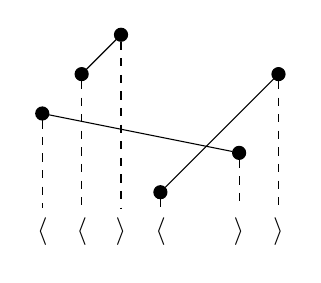
\begin{tikzpicture}[scale=0.5]
\tikzstyle{dot}=[draw,shape=circle,fill=black,scale=0.5]
\node[dot] at (0,2) (p1) {};
\node[dot] at (1,3) (p2) {};
\node[dot] at (2,4) (p3) {};
\node[dot] at (3,0) (p4) {};
\node[dot] at (5,1) (p5) {};
\node[dot] at (6,3) (p6) {};

\node at (0,-1) (b1) {$\langle$};
\node at (1,-1) (b2) {$\langle$};
\node at (2,-1) (b3) {$\rangle$};
\node at (3,-1) (b4) {$\langle$};
\node at (5,-1) (b5) {$\rangle$};
\node at (6,-1) (b6) {$\rangle$};

\draw (p1) -- (p5);
\draw (p2) -- (p3);
\draw (p4) -- (p6);

\draw[dashed] (p1) -- (b1);
\draw[dashed] (p2) -- (b2);
\draw[dashed] (p3) -- (b3);
\draw[dashed] (p4) -- (b4);
\draw[dashed] (p5) -- (b5);
\draw[dashed] (p6) -- (b6);
\end{tikzpicture}}
Construct a bracket expression $\bracketing_{\pointset P}\of\gm$ of length $n$ as follows: order $\pointset P$ from left
to right;
the $i$th bracket is opening if the $i$th point of $\pointset P$ is a left endpoint of $\gm$, and it is
closing otherwise.
This bracket expression is well-formed, since it can be constructed by starting from the
(well-formed) empty bracket expression, by successively inserting both brackets corresponding to
each edge, where the closing bracket will be inserted to the right of the opening bracket.

Given a well-formed bracket expression $B$ and a point set $\pointset P$, we will say that a perfect matching
$\gm$ is \emph{consistent with} $B$ if $\bracketing_{\pointset P}\of\gm = B$; moreover, we will refer to the points of
$\pointset P$ corresponding to opening brackets of $B$ as \emph{left-points} (since they will be left endpoints
of any perfect matching consistent with $B$), and similarly we will refer to the points of $\pointset P$
corresponding to closing brackets of $B$ as \emph{right-points}.

One approach to bounding the size of $\CFPM_{\pointset P}$ is to bound the size of
$\bracketing_{\pointset P}^{-1}\of{B}\Intersection \CFPM_{\pointset P}$ for bracket expressions $B$ of length $n$\idest the
number of crossing-free perfect matchings on $\pointset P$ consistent with $B$. We thus define
\[\gn_{\pointset P}\of B \DefineAs
\Cardinality{\bracketing_{\pointset P}^{-1}\of{B}\Intersection \CFPM_{\pointset P}}\text.\]
In order to concisely refer to bracket expressions, we will use the notations
$\langle^k$ for $k$ successive opening brackets, and $\rangle^k$ for $k$ successive
closing brackets, for instance,\[
\langle^2\rangle\langle^2\rangle^3 = \langle\langle\rangle\langle\langle\rangle\rangle\rangle
\text.\]

A remarkable property of $\gn$ is its behaviour with respect to concatenation of well-formed bracket expressions.
If $B_1$ and $B_2$ are well-formed bracket expressions of lengths $k_1$ and $k_2=n-k_1$,
$\pointset P_1$ is the set of the leftmost $k_1$ points of $\pointset P$, and
$\pointset P_2=\pointset P\setminus\pointset P_1$ is the set of the
rightmost $k_2$ points, we have\[
\gn_{\pointset P}\of{B_1B_2}=\gn_{\pointset P_1}\of{B_1}\gn_{\pointset P}\of{B_2}\text.
\]
Indeed, no edge may join $\pointset P_1$ and $\pointset P_2$, since half the points of $\pointset P_1$ are right-points,
and $\pointset P_1$ lies to the left of $\pointset P_2$. The problem thus decomposes in two independent parts.

The function $\gn_{\pointset P}$ has been studied before; though they did not explicitly phrase it in terms of brackets,
M.~Sharir and E.~Welzl showed in 2005 \cite{SharirWelzl2006} that\begin{equation}
\gn_{\pointset P}\of B\preccurlyeq_n5.3793^n
\label{boundOnLeftRightPerfectMatchings}
\end{equation}
uniformly in $B$. Taking the sum of this bound over bracket expressions $B$ yields an upper bound for the overall number of
crossing-free perfect matchings,\[
\Cardinality{\CFPM_{\pointset P}}
\preccurlyeq_n \CatalanNumber {\frac n 2} 5.3793^n
\preccurlyeq_n 10.76^n\text,
\]
but it is worse than the one mentioned in the previous section.
\subsectionorsection{An optimal lower bound for the number of crossing-free perfect matchings}
The following result, and its proof are, due to A.~J.~Ruiz-Vargas and E.~Welzl \cite{RuizVargasWelzl2016}.
\begin{theorem}[Ruiz-Vargas--Welzl]
Let $\pointset P$ be a point set of size $n = 2k$ in general position with respect to the horizontal,
and let $B$ be a well-formed bracket expression of length $n$.
Then there exists a crossing-free perfect matching consistent with $B$; in other words,
$\gn_{\pointset P}\of B \geq 1$.
\end{theorem}
\begin{proof}
Let $\gm_0$ be a perfect matching on $\pointset P$ consistent with $B$. This is always possible, for instance,
parsing the bracket expression, match the point corresponding to an opening bracket
and the point corresponding to the matching closing bracket.

Define $\gL\of\gm$ for a perfect matching $\gm$ on $\pointset P$ to be the sum of the lengths of the edges of $\gm$.

\marginfig[\label{figUncrossing}Untangling in a perfect matching. Replacing the thick
edges by the thin ones reduces the total edge length, while preserving left and right endpoints.]{
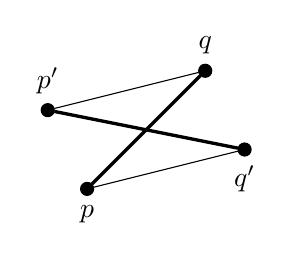
\begin{tikzpicture}[scale=1]
\tikzstyle{dot}=[draw,shape=circle,fill=black,scale=0.5]
\node[dot,label=below:$p$] at (0,0) (a) {};
\node[dot,label=above:$p'$] at (-0.5,1) (c) {};
\node[dot,label=below:$q'$] at (2,0.5) (d) {};
\node[dot,label=above:$q$] at (1.5,1.5) (b) {};

\draw (a) -- (d);
\draw (c) -- (b);
\draw[very thick] (a) -- (b);
\draw[very thick] (c) -- (d);
\end{tikzpicture}}
Then, repeat the following procedure, starting at $i=0$.
If there is no crossing in $\gm_i$, we have found a perfect matching with the desired properties.
If there is a crossing, let $p$, $p'$, $q$, and $q'$ be the points involved, with $p$ and $p'$ being the left
endpoints and $q$ and $q'$ being the right endpoints, so that the edge
$pq$ crosses the edge $p'q'$. Remove these edges, and replace them by $pq'$ and $p'q$, thus untangling them.
This yields another perfect matching $\gm_{i+1}$. By the triangle
inequality (see figure \ref{figUncrossing}), $\gL\of{\gm_{i+1}}<\gL\of{\gm_i}$.

If this procedure did not terminate, it would yield a sequence $\tuple{\gm_i}_{i\in\N}$ of crossing
perfect matchings on $\pointset P$ on which $\gL$ is strictly decreasing, thus an infinite sequence of distinct
graphs on $\pointset P$.
Since there are only finitely many graphs on $\pointset P$, this is a contradiction, so we
eventually\footnote{The untangling procedure itself predates this proof, and was shown to terminate in
$\BigO\of{n^3}$ steps by J.~van~Leeuwen and A.~A.~Schoone in 1980 \cite{LeeuwenSchoone1981}.}
find a
crossing-free perfect matching.
\end{proof}
This immediately yields a lower bound for the number of crossing-free perfect matchings, since
there are $\CatalanNumber {\frac n 2}$ well-formed bracket expressions of length $n$.
Note that this lower bound had already been proved by A.~García, M.~Noy, and J.~Tejel in 1995,
by a recurrence that split the point set, yielding the Segner recurrence with inequality,
rather than via well-formed bracket expressions
\cite{GarciaNoyTejel2000}.
\begin{corollary}
Let $\pointset P$ be a point set of even size $n$ in general position. There are at least $\CatalanNumber {\frac n 2}$ distinct
crossing-free perfect matchings on $\pointset P$\idest $\Cardinality{\CFPM_{\pointset P}} \geq \CatalanNumber {\frac n 2}$.
\end{corollary}
Moreover, this lower bound is optimal, since it is attained if $\pointset P$ is in convex position (see
section~\ref{PerfectMatchingsIntro}).

Now that we have a tight uniform lower bound for $\gn_{\pointset P}$, we will start looking at upper bounds
dependent on the bracket expression.
\subsectionorsection{Matchings across a line}\label{MatchingsAcrossALine}
Again we consider $n=2k$ points in general position with respect to the horizontal.
The matchings consistent with bracket expressions with $k$ opening brackets followed
by $k$ closing brackets, $\langle^k\rangle^k$, are called \emph{matchings
across a line}. Indeed, any edge in such a matching will cross any vertical line that separates
the left-points from the right-points.

The following result, and its proof, were given by M.~Sharir and E.~Welzl in 2005 \cite{SharirWelzl2006}.
\NoEndMark
\begin{theorem}[Sharir--Welzl]\label{thmCFPMAL}
Let $\pointset P$ be a set of $n=2k$ points in general position with respect to the horizontal.
Then there are at most ${\CatalanNumber {\frac n 2}}^2$ crossing-free perfect matchings across a line on $\pointset P$\idest
$\gn_{\pointset P}\of {\langle^k\rangle^k} \leq {\CatalanNumber k}^2$.
\end{theorem}
The idea of the proof is as follows.
First, pick a vertical line that separates the left-points from the right-points;
we will call it \emph{the vertical line}.
Further, let us call the set of left-points $\pointset L$ and the set of right-points $\pointset R$.

A perfect matching consistent with a given well-formed bracket expression (and in particular, a perfect
matching across a line) is uniquely defined by a bijection $\FunctionSpec \gm {\pointset L} {\pointset R}$ from
the left-points to the right-points. Consider such a perfect
matching across a line, and let $E$ be the set of its edges.
Now, number the intersections between the edges of the perfect matching and the vertical
line from top to bottom. This yield a numbering $\FunctionSpec \gi E {[k]}$ of the edges.
\marginfig[Constructing the numberings $\gl$ and $\gr$ of the left- and right-points from
a crossing-free perfect matching across a line; here $\gi\of{\set{p,q}} = 2$, and thus
$\gl\of{p}=\gr\of q = 2$.\label{figConstructCFA}]{
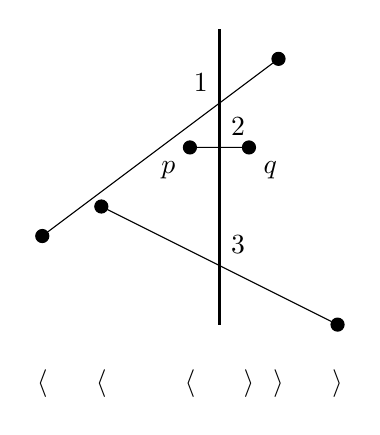
\begin{tikzpicture}[scale=0.75]
\tikzstyle{dot}=[draw,shape=circle,fill=black,scale=0.5]
\node[dot] at (-3,1.5) (l1) {};
\node[dot] at (-2,2) (l2) {};
\node[dot,label=below left:$p$] at (-0.5,3) (l3) {};
\node[dot,label=below right:$q$] at (0.5,3) (r1) {};
\node[dot] at (1,4.5) (r2) {};
\node[dot] at (2,0) (r3) {};

\node at (-3,-1) {$\langle$};
\node at (-2,-1) {$\langle$};
\node at (-0.5,-1) {$\langle$};
\node at (0.5,-1) {$\rangle$};
\node at (1,-1) {$\rangle$};
\node at (2,-1) {$\rangle$};

\node[inner sep=0pt,label=above left:$1$] at (0,3.75) {};
\node[inner sep=0pt,label=above right:$2$] at (0,3) {};
\node[inner sep=0pt,label=above right:$3$] at (0,1) {};

\draw (l1) -- (r2);
\draw (l2) -- (r3);
\draw (l3) -- (r1);

\draw[very thick] (0,5) -- (0,0);
\end{tikzpicture}}

Define $\gl\of p \DefineAs \gi\of{e_p}$ mapping a left-point to the intersection number of its
edge, and similarly $\gr\of q \DefineAs \gi\of{e_q}$ for the right-points. We have
$\gm = \gr^{-1} \Compose \gl$.
The bijection $\gl$ (respectively $\gr$) determines the order in which the left points (respectively right points)
reach the vertical line.

If the matching is crossing-free, we will show that
$\gl$ and $\gr$ have to be in sets of size $\CatalanNumber k$, thus that there are at most ${\CatalanNumber k}^2$ functions
$\gm = \gr^{-1} \Compose \gl$\idest that there can be at most ${\CatalanNumber k}^2$ crossing-free perfect matchings across a line.

Since we are going to reuse these concepts in subsequent \sectionsorchaptersword, we will formalize and name the properties of
$\gl$ and $\gr$ that we will consider.
\begin{definition}[crossing-free alignment]
Let ${\pointset S}$ be a set of $k$ points in general position. Let $V$ be a vertical line to the right of ${\pointset S}$.
A bijection $\gl$ from ${\pointset S}$ to $[k]$ is a \emph{crossing-free left-alignment of ${\pointset S}$ on $V$} if
there exists a set $A=\setst{\gs_p}{p\in{\pointset S}}$ of $k$ line segments such that
the following hold:
\begin{enumerate}
\item for every $p\in{\pointset S}$, the left endpoint of $\gs_p$ is $p$, and its right endpoint is on $V$;
\item no two segments cross, and no two segments share any endpoints;
\item let $\FunctionSpec \gi A {[k]}$ the numbering of the right endpoints of the segments in
$A$ from top to bottom, then $\gl\of p = \gi\of{\gs_p}$.
\end{enumerate}
Such a set of segments is said to \emph{realize} $\gl$.

Correspondingly, we define a \emph{crossing-free right-alignment}, where ``right'' and ``left'' are swapped in the
definition.
\end{definition}
\begin{sloppypar}
A crossing-free left-alignment of five points, with a realizing set of segments---drawn as arrows---is shown in
figure~\ref{figCrossingFreeAlignment}.
\end{sloppypar}

\marginfig[A crossing-free left-alignment of five points. Once the index of the leftmost point is chosen (thick segment),
the rest consists of two crossing-free left-alignments of $i$ and $k-i-1$
points each---here $k = 5$ and $i = 2$.\label{figCrossingFreeAlignment}]{
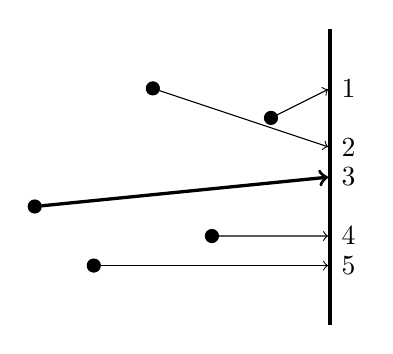
\begin{tikzpicture}[scale=0.75]
\tikzstyle{dot}=[draw,shape=circle,fill=black,scale=0.5]
\node[dot] at (-5,2) (p1) {};
\node[dot] at (-4,1) (p2) {};
\node[dot] at (-3,4) (p3) {};
\node[dot] at (-2,1.5) (p4) {};
\node[dot] at (-1,3.5) (p5) {};

\node[inner sep=0pt,label=right:$1$] at (0,4) (l1) {};
\node[inner sep=0pt,label=right:$2$] at (0,3) (l2) {};
\node[inner sep=0pt,label=right:$3$] at (0,2.5) (l3) {};
\node[inner sep=0pt,label=right:$4$] at (0,1.5) (l4) {};
\node[inner sep=0pt,label=right:$5$] at (0,1) (l5) {};

\draw[->,very thick] (p1) -- (l3);
\draw[->] (p3) -- (l2);
\draw[->] (p5) -- (l1);
\draw[->] (p4) -- (l4);
\draw[->] (p2) -- (l5);

\draw[very thick] (0,5) -- (0,0);
\end{tikzpicture}}
\begin{lemma}
Let ${\pointset S}$ be a set of $k$ points in general position, and let $V$ be a vertical line to the right of ${\pointset S}$.
There are at most $\CatalanNumber k$ crossing-free left-alignments of ${\pointset S}$ on $V$.
\begin{proof}
Let $\gl$ be a crossing-free left-alignment of ${\pointset S}$ on $V$.
Let $A=\setst{\gs_p}{p\in{\pointset S}}$ be a set of non-crossing line segments realizing $\gl$.
For a point $p\in{\pointset S}$, we will call $\gs_p$ \emph{the segment of $p$}.

$\gl(\leftmost\pointset S)$, being the index on the vertical line $V$ of the right endpoint of the
segment $\gs_{\leftmost\pointset S}$
of the leftmost point,
is equal to $1$ plus the number of points of ${\pointset S}$ that are above $\gs_{\leftmost\pointset S}$.
Indeed, the segments of points above $\gs_{\leftmost\pointset S}$ must
themselves reach the vertical line $V$ above $\gs_{\leftmost\pointset S}$,
otherwise they would cross $\gs_{\leftmost\pointset S}$, and correspondingly for
points below $\gs_{\leftmost\pointset S}$,
so that there are as many edges reaching the vertical line $V$ below $\gs_{\leftmost\pointset S}$ as there are points
below $\gs_{\leftmost\pointset S}$.

\begin{sloppypar}
Moreover, as the oriented angle between $\gs_{\leftmost\pointset S}$
and the horizontal increases, points are only added to the
set of points below $\gs_{\leftmost\pointset S}$, so that choosing the number of points below
$\gs_{\leftmost\pointset S}$ determines the sets of points
below and above $\gs_{\leftmost\pointset S}$.
\end{sloppypar}

Further, since points above $\gs_{\leftmost\pointset S}$ must reach the vertical line $V$ above
$\gs_{\leftmost\pointset S}$, and correspondingly for points below,
if the point $p$ is above $\gs_{\leftmost\pointset S}$, then $\gl(p) < \gl({\leftmost\pointset S})$,
and if it is below, $\gl(p) > \gl({\leftmost\pointset S})$. Thus
$\gl$ restricted to the points above $\gs_{\leftmost\pointset S}$ is a crossing-free left-alignment of
the $\gl({\leftmost\pointset S}) - 1$ points above
$\gs_{\leftmost\pointset S}$, and $\gl-\gl({\leftmost\pointset S})$ restricted to the points below
$\gs_{\leftmost\pointset S}$ is a crossing-free left-alignment of the
$k - \gl({\leftmost\pointset S})$ points below $\gs_{\leftmost\pointset S}$,
where the appropriate subsets of $A$ provide the set of segments required
in the definition.

It follows that $\gl$ is determined by the choice of $\gl\of {\leftmost\pointset S}$
and crossing-free left-align\-ments
of $\gl\of{\leftmost\pointset S}-1$ and $k-\gl\of{\leftmost\pointset S}$ points.
Letting $i\DefineAs \gl\of {\leftmost\pointset S} - 1$, these are crossing-free alignments of $i$ and $k-i-1$ points (see
figure~\ref{figCrossingFreeAlignment}).
Therefore, if $\gcp_j$ is an upper bound for the number of crossing-free
left-alignments of $j$ points when $j < k$,
we can give an upper bound on the number of crossing-free left-alignments of $k$ points,
\[\gcp_k\DefineAs\sum{i=0}[k-1]\gcp_{i}\gcp_{k-i-1}\text.\]
We can start the recurrence with $\gcp_0 = 1$; this is the recurrence for the Catalan numbers, thus
$\gcp_k=\CatalanNumber k$.
\end{proof}
\end{lemma}
The same result holds for crossing-free right-alignments, simply exchange ``left'' and ``right'' in the above
lemma and its proof.

\begin{proof}[\eggorcadmo{of the theorem}{of theorem~\ref{thmCFPMAL}}]
If we have a crossing-free perfect matching across a line, then $\gl$ as constructed in figure~\ref{figConstructCFA}
is a crossing-free
left-alignment of $\pointset L$ on the vertical line; indeed, letting $\gs_p$ be the portion of the edge $e_p$
to the left of the vertical line yields segments that realize $\gl$.
Similarly, $\gr$ is a crossing-free right-alignment of $\pointset R$ on the vertical line.
\end{proof}

\sectionorchapter{Analysing the overcounting in the upper bound for matchings across a line}
\label{sectionOvercounting}
\marginfig[Composing crossing-free alignments, only to get a crossing perfect
matching.\label{figCrossingPMAL}]{
\begin{tikzpicture}[scale=0.6]
\tikzstyle{dot}=[draw,shape=circle,fill=black,scale=0.5]

\draw[very thick, name path=V] (0,1.5) -- (0,-2);

\node[dot] at (-3,1) (l1) {};
\node[dot] at (-1,0.25) (l2) {};

\node[dot] at (1,1) (r1) {};
\node[dot] at (3,0) (r2) {};

\coordinate (a1) at (0,0);
\coordinate (a2) at (0,-1.5);

\draw (l1)--(r2);
\draw (l2)--(r1);

\draw[->,very thick] (l1) -- (a2);
\draw[->,very thick] (r2) -- (a2);
\draw[->,very thick] (r1) -- (a1);
\draw[->,very thick] (l2) -- (a1);
\end{tikzpicture}}
\marginfig[Composing crossing-free alignments, and getting a crossing-free perfect matching,
but one that does not decompose to the original alignments.\label{figWeirdAligments}]{
\begin{tikzpicture}[scale=0.6]
\tikzstyle{dot}=[draw,shape=circle,fill=black,scale=0.5]

\draw[very thick, name path=V] (0,2) -- (0,-2);

\node[dot] at (-3,1) (l1) {};
\node[dot] at (-1,0.25) (l2) {};

\node[dot] at (1,1) (r1) {};
\node[dot] at (3,1.5) (r2) {};

\coordinate (a1) at (0,0);
\coordinate (a2) at (0,-1.5);

\draw (l1)--(r2);
\draw (l2)--(r1);

\draw[->,very thick] (l1) -- (a2);
\draw[->,very thick] (r2) -- (a2);
\draw[->,very thick] (r1) -- (a1);
\draw[->,very thick] (l2) -- (a1);
\end{tikzpicture}}
The bound given in the previous \sectionorchapterword for the number of matchings across a line is not optimal;
an example is given by Sharir and Welzl of a crossing-free left-alignment $\gl$ and a crossing-free
right-alignment $\gr$ such that $\gr^{-1}\Compose \gl$ is not crossing-free (see figure~\ref{figCrossingPMAL}).

There is however more to the overcounting than just counting some crossing matchings.
To characterize that, it helps to name some functions and sets. Again, we are considering a
set $\pointset P$ of $2k$ points in general position with respect to the horizontal and the bracket
expression $\langle^k\rangle^k$.  We let $\pointset L$ be the set of left-points, and $\pointset R$ be the
set of right-points. Moreover, we pick a vertical line $V$ separating $\pointset L$ and $\pointset R$.
In this \sectionorchapterword and the following one, we will use the terms crossing-free left- and right-alignments
to mean crossing-free left- and right-alignments on $V$.

\begin{sloppypar}
In the previous \sectionorchapterword, given a crossing-free perfect matching $\gm$, we constructed crossing-free
left- and right-alignments $\gl$ and $\gr$ (see figure~\ref{figConstructCFA}). Let us call these
crossing-free alignments the \emph{decomposition} $\decomposition$ of $\gm$,
thus $\decomposition\of{\gm}=\tuple{\gl, \gr}$.
We remarked that the composition $\gr^{-1}\Compose\gl$ of these alignments yielded the original matching.
We thus define the \emph{composition} $\composition\of{\gl,\gr}\DefineAs\gr^{-1}\Compose\gl$ for
arbitrary crossing-free left-aligment $\gl$ of $\pointset L$ on $V$ and $\gr$ of $\pointset R$ on $V$.
Moreover, let us call $\CFLA_{\pointset L, V}$ the
set of crossing-free left-alignments of $\pointset L$ on $V$, and $\CFLA_{\pointset R, V}$ the set of crossing-free
left-alignments of $\pointset R$ on $V$.
Finally, let us name the sets of perfect matchings across a line and of
crossing-free perfect matchings across a line,
\begin{align*}
\PMAL_{\pointset P} &\DefineAs \bracketing_{\pointset P}^{-1}\of{\langle^k\rangle^k}\\
\CFPMAL_{\pointset P} &\DefineAs \PMAL_{\pointset P} \Intersection \CFPM_{\pointset P}\text.
\end{align*}
Then the following diagram commutes\idest decomposing a crossing-free perfect matching across a line
and then composing the resulting alignments yields the initial matching.
\[\begin{tikzcd}
\CFPMAL_{\pointset P} \arrow{r}{\decomposition} \arrow[hook]{d}{\Subset} &
\CFLA_{\pointset L, V}\Cartesian\CFRA_{\pointset R, V} \arrow{ld}{\composition} \\
\PMAL_{\pointset P}
\end{tikzcd}\]
We will call the elements of $\CFLA_{\pointset L, V}\Cartesian\CFRA_{\pointset R, V}$ \emph{pairs of alignments}.
\end{sloppypar}

The result of Sharir and Welzl is proved in two steps. First we see
from the commutative diagram that $\CFPMAL_{\pointset P}$ lies within the image of
$\composition$, so that\begin{align}
\gn_{\pointset P}\of{\langle^k\rangle^k} &=
\Cardinality{\CFPMAL_{\pointset P}} \nonumber \\ &\leq
\Cardinality{\composition\of{\CFLA_{\pointset L, V}\Cartesian\CFRA_{\pointset R, V}}} \nonumber \\ &\leq
\Cardinality{\CFLA_{\pointset L, V}\Cartesian\CFRA_{\pointset R, V}}\text. \label{SharirWelzlOvercounting}
\end{align}
Then, we derive an upper bound for the number $\Cardinality{\CFLA_{\pointset L, V}\Cartesian\CFRA_{\pointset R, V}}$
of pairs of alignments. We will examine this second step later.
Looking at the commutative diagram, we can see that $\decomposition$ is injective; this is another way of getting
(\ref{SharirWelzlOvercounting}), but more importantly, it means that $\gn_{\pointset P}\of{\langle^k\rangle^k}$
is equal to the cardinality of the image of $\decomposition$.

It follows that the pairs of alignments that are \emph{not} in the image of $\decomposition$ are responsible
for the slackness of the inequality (\ref{SharirWelzlOvercounting}). We will thus call them
\emph{overcounted pairs of alignments}.
An overcounted pair of alignments $\tuple{\gl,\gr}$ falls into one of two families:
\begin{enumerate}
\item
$\composition\of{\gl,\gr}$ can be a crossing perfect matching, as in figure~\ref{figCrossingPMAL};
\item $\composition\of{\gl,\gr}$ can be a crossing-free perfect matching;
in this case, we have $\tuple{\gl,\gr}\neq\decomposition\Compose\composition\of{\gl,\gr}$,
since $\tuple{\gl,\gr}$ is overcounted; an example is shown in figure~\ref{figWeirdAligments}.
\end{enumerate}
\marginfig[A set $\pointset S$ of five points. The half-plane to the right
of the leftmost point $\leftmost \pointset S$ is partitioned into
$\Cardinality{\pointset S}$ cones $\scone i$.\label{figCones}]{
\begin{tikzpicture}[scale=0.75]
\tikzstyle{dot}=[draw,shape=circle,fill=black,scale=0.5]
\shade[shading=axis,
       left color=gray,
       right color=white] (-5,0) rectangle (0,5);
       
\node[dot, label=left:$\leftmost \pointset S$] at (-5,2) (lm) {};
\node[dot] at (-4,1) (p2) {};
\node[dot] at (-3,4) (p3) {};
\node[dot] at (-2,1.5) (p4) {};
\node[dot] at (-1,3.5) (p5) {};

\node at (-4.5,0.5) {$\scone 5$};
\node at (-2.5,1) {$\scone 4$};
\node at (-1.5,2.5) {$\scone 3$};
\node at (-2,4) {$\scone 2$};
\node at (-4,4) {$\scone 1$};

\draw (-5,5) -- (-5,0);

\begin{scope}
\clip (-5,0) rectangle (0,5);
\draw (lm) -- ($(lm)!10cm!(p2)$);
\draw (lm) -- ($(lm)!10cm!(p3)$);
\draw (lm) -- ($(lm)!10cm!(p4)$);
\draw (lm) -- ($(lm)!10cm!(p5)$);
\end{scope}
\end{tikzpicture}}
\marginfig[A crossing-free perfect matching $\gm$ across a line $V$.
Its decomposition is $\tuple{\gl,\gr}\DefineAs\decomposition\of\gm$;
the crossing-free left-alignment $\gl$ is shown here. Since
$\gl\of{\leftmost\pointset L}=3$, $\leftmost\pointset L$ is matched within
the cone $\lcone 3$ (shaded).\label{figConesNeedPoints}]{
\begin{tikzpicture}[scale=0.6]
\tikzstyle{dot}=[draw,shape=circle,fill=black,scale=0.5]

\draw[very thick, name path=V] (0,5) -- (0,0);

\node at (-2,5) {$\pointset L$};

\node at (0,5.5) {$V$};

\node at (1,5) {$\pointset R$};

\node[dot] at (-.5,4.5) (a1) {};
\node[dot] at (-1,3.5) (a3) {};
\node[dot,label=left:$\leftmost\pointset L$] at (-4,3) (a4) {};
\node[dot] at (-1.3,2) (a6) {};

\node[dot] at (2,4.7) (b1) {};
\node[dot] at (1.5,2.6) (b3) {};
\node[dot] at (2.5,1.8) (b4) {};
\node[dot] at (1,0.5) (b6) {};

\draw[gray, name path=edge] (a1) -- (b1);
\draw[->,thick,name intersections={of=edge and V, by=align}] (a1) -- (align);
\node[label={[font=\scriptsize,label distance=-5pt]below left:$1$}] at (align) {};
\draw[gray, name path=edge] (a3) -- (b3);
\draw[->,thick,name intersections={of=edge and V, by=align}] (a3) -- (align);
\node[label={[font=\scriptsize,label distance=-5pt]below left:$2$}] at (align) {};
\draw[gray, name path=edge] (a4) -- (b4);
\draw[->,thick,name intersections={of=edge and V, by=align}] (a4) -- (align);
\node[label={[font=\scriptsize,label distance=-5pt]below left:$3$}] at (align) {};
\draw[gray, name path=edge] (a6) -- (b6);
\draw[->,thick,name intersections={of=edge and V, by=align}] (a6) -- (align);
\node[label={[font=\scriptsize,label distance=-5pt]below left:$4$}] at (align) {};

\begin{scope}
\clip (-4,0) rectangle (2.5,5);
\draw[dotted] (-4,0) -- (-4,5);
\draw[dotted] (a4) -- ($(a4)!10cm!(a1)$);
\draw[dotted] (a4) -- ($(a4)!10cm!(a3)$);
\draw[dotted] (a4) -- ($(a4)!10cm!(a6)$);
\end{scope}

\begin{scope}[on background layer]
\clip ($(a4)!10cm!(a3)$) -- (a4.center) -- ($(a4)!10cm!(a6)$) -- cycle;
\shade[shading=axis,
       left color=gray,
       right color=white] (-5,0) rectangle (2.5,6);
\end{scope}
\end{tikzpicture}}

We would like to give a bound on the number of non-overcounted pairs of alignments. In order to do that,
we turn to the second part of the proof of Sharir and Welzl, namely the bound on the number of pairs of alignments,
and examine it in more detail, with some fresh definitions. Again, we will look at crossing-free left-alignments; the
following argument equally applies to crossing-free right-alignments.

For a point set $\pointset S$ in general position with respect to the horizontal,
note that we can partition the half-plane to the right of $\leftmost\pointset S$ into
$\Cardinality{\pointset S}$ regions,
separated by rays emanating from $\leftmost\pointset S$ and going through other points of
$\pointset S$, see figure~\ref{figCones}.
We will call those regions, from top to bottom, $\scone 1$ to
$\scone {\Cardinality{\pointset S}}$.
Note that there are $i$ points of $\pointset S$ above the interior of $\scone {i+1}$,
and $\Cardinality {\pointset S} - i - 1$ points below.
We will use the term \emph{left cone of $\pointset L$} to mean
$\scone {i}$ for some $\pointset S\Subset\pointset L$ and some $i\in[\pointset S]$.

Observe that for a crossing-free left-alignment $\gl$ of $\pointset L$ with
$\gl\of{\leftmost\pointset L} = i+1$,
any realizing segment of $\gl$ incident to $\leftmost\pointset L$
separates the points $\pointset L\setminus\set{\leftmost\pointset L}$ into sets of points above and below the
segment, as in figure~\ref{figCrossingFreeAlignment}. Furthermore, these sets are the same as the sets of points
above and below $\lcone {i+1}$.
As a consequence, given a crossing-free left-alignment
$\gl$ of $\pointset L$, for any set of segments $A=\setst{\gs_p}{p\in\pointset L}$
realizing $\gl$, the segment $\gs_{\leftmost\pointset L}$ of the leftmost point has to be contained in
$\lcone{\gl\of{\leftmost\pointset L}}$.
As we remarked in section~\ref{MatchingsAcrossALine}, for a crossing-free perfect matching
$\gm$, the edges of $\gm$ restricted to the left side of $V$ realize the crossing-free
left-alignment in $\decomposition\of\gm$. Thus, if $\tuple{\gl, \gr}=\decomposition\of\gm$ is in the image of
$\decomposition$, $\gm$ must match $\leftmost\pointset L$ to a right-point in the cone
$\lcone{\gl\of{\leftmost\pointset L}}$, see figure~\ref{figConesNeedPoints}.

To extend this reasoning beyond the leftmost point of $\pointset L$, we define \emph{left conifers\footnote{Conifers are
constructed by recursive subdivision, so in some sense they are trees with cones, hence the name.}
on $\pointset L$}.
A left conifer $\gk$ on $\pointset L$ is a map from points in $\pointset L$ to left
cones of $\pointset L$,
satisfying the following properties:
\begin{enumerate}
\item $\gk\of{\leftmost\pointset L}$ is a left $\pointset L$-cone;
\item $\gk$ restricted to the points above the interior of $\gk\of{\leftmost\pointset L}$ is a left conifer on these points;
\item $\gk$ restricted to the points below the interior of $\gk\of{\leftmost\pointset L}$ is a left conifer on these points.
\end{enumerate}
See figure~\ref{figLeftConifer} for an example.
\begin{figure}[ht!]
\centering
\begin{subfigure}{.45\textwidth}
  \centering
\begin{tikzpicture}[scale=0.75]
\tikzstyle{dot}=[draw,shape=circle,scale=0.5]
       
\node[dot,fill=red, label=above:$\leftmost\pointset L$] at (-5,2) (lm) {};
\node[dot,fill=white] at (-4,1) (p2) {};
\node[dot,fill=black] at (-3,4) (p3) {};
\node[dot,fill=white] at (-2,1.5) (p4) {};
\node[dot,fill=black] at (-1,3.5) (p5) {};

\begin{scope}[on background layer]
\begin{scope}
\clip ($(lm)!10cm!(p5)$) -- (lm.center) -- ($(lm)!10cm!(p4)$) -- cycle;
\shade[shading=axis,
       left color=red,
       nearly transparent] (-5,0) rectangle (0,5);
\end{scope}
\end{scope}
\end{tikzpicture}
  \caption{The conifer maps the leftmost point of $\pointset L$ to an $\pointset L$-cone,
  in this case $\lcone 3$.
  This separates the other points into those above (black) and below (white) the interior of $\lcone 3$.
  The construction is continued by constructing left conifers on both subsets.}
\end{subfigure}\hfill
\begin{subfigure}{.45\textwidth}
  \centering
\begin{tikzpicture}[scale=0.75]
\tikzstyle{dot}=[draw,shape=circle,scale=0.5]
       
\node[dot,fill=red] at (-5,2) (lm) {};
\node[dot,fill=green] at (-4,1) (p2) {};
\node[dot,fill=blue] at (-3,4) (p3) {};
\node[dot,fill=cyan] at (-2,1.5) (p4) {};
\node[dot,fill=black] at (-1,3.5) (p5) {};

\begin{scope}[on background layer]
\begin{scope}
\clip ($(lm)!10cm!(p5)$) -- (lm.center) -- ($(lm)!10cm!(p4)$) -- cycle;
\shade[shading=axis,
       left color=red,
       nearly transparent] (-5,0) rectangle (0,5);
\end{scope}
\begin{scope}
\clip ($(p2)!10cm!(p4)$) -- (p2.center) -- (-4,0) -- (0,0) -- cycle;
\shade[shading=axis,
       left color=green,
       nearly transparent] (-4,0) rectangle (0,5);
\end{scope}
\begin{scope}
\clip ($(p3)!10cm!(p5)$) -- (p3.center) -- (-3,0) -- (0,0) -- cycle;
\shade[shading=axis,
       left color=blue,
       nearly transparent] (-3,0) rectangle (0,5);
\end{scope}
\shade[shading=axis,
       left color=cyan,
       nearly transparent] (-2,0) rectangle (0,5);
\shade[shading=axis,
       left color=black,
       nearly transparent] (-1,0) rectangle (0,5);
\end{scope}
\end{tikzpicture}
  \caption{The completed left conifer; the cone associated with each point is drawn in the same colour
  as that point.}
\end{subfigure}
\caption{The construction of a left conifer on a set $\pointset L$ of five points.}
\label{figLeftConifer}
\end{figure}

Let $\LC {\pointset L}$ be the set of left conifers on $\pointset L$. From the observations above on the number
of cones and the
size of the sets of points above and below their interiors, we can see that the number of left conifers on a point
set depends only on the size of that point set. Specifically, if $\gcp_k$ is the number of left conifers on $k$ points,
we have
\[
\gcp_k=\sum{i=0}[k-1]\gcp_{i}\gcp_{k-i-1} \text{ and } \gcp_0=1\text,
\]
where the summation index $i$ corresponds to the choice $\gk\of{\leftmost L}=\lcone {i+1}$.
We thus have $\Cardinality{\LC {\pointset L}} = \CatalanNumber {\Cardinality{\pointset L}}$.

Recall that a crossing-free left-alignment $\gl$ of $\pointset L$ on $V$
is determined by the value of $\gl\of{\leftmost\pointset L}$ and by
crossing-free left alignments $\gl^-$ and $\gl^+$ on $V$
of subsets $\pointset S^-$ and $\pointset S^+$ above and below any edge
realizing $\gl$ incident to $\leftmost\pointset L$\idest subsets above
and below $\lcone{\gl\of{\leftmost\pointset L}}$. In other words, we have
\begin{align*}
\pointset S^- &= \gl^{-1}\of{\set{1,\dotsc,\gl\of{\leftmost\pointset L}-1}}\text,\\
\pointset S^+ &= \gl^{-1}\of{\set{\gl\of{\leftmost\pointset L}+1,\dotsc,\Cardinality{\pointset L}}}\text,\\
\gl^-\of{p} &= \gl\of{p} \text{ for $p\in\pointset S^-$, and}\\
\gl^+\of{p} &= \gl\of{p}-\gl\of{\leftmost\pointset L} \text{ for $p\in\pointset S^+$.}
\end{align*}

\marginfig[A crossing-free left-alignment $\gl$ (the one from figure~\ref{figCrossingFreeAlignment}),
together with the conifer $\conification_\gl$.\label{figConification}]{
\begin{tikzpicture}[scale=0.75]
\tikzstyle{dot}=[draw,shape=circle,scale=0.5]
       
\node[dot,fill=red] at (-5,2) (lm) {};
\node[dot,fill=green] at (-4,1) (p2) {};
\node[dot,fill=blue] at (-3,4) (p3) {};
\node[dot,fill=cyan] at (-2,1.5) (p4) {};
\node[dot,fill=black] at (-1,3.5) (p5) {};

\node[inner sep=0pt,label=right:$1$] at (0,4) (l1) {};
\node[inner sep=0pt,label=right:$2$] at (0,3) (l2) {};
\node[inner sep=0pt,label=right:$3$] at (0,2.5) (l3) {};
\node[inner sep=0pt,label=right:$4$] at (0,1.5) (l4) {};
\node[inner sep=0pt,label=right:$5$] at (0,1) (l5) {};

\draw[->] (lm) -- (l3);
\draw[->] (p3) -- (l2);
\draw[->] (p5) -- (l1);
\draw[->] (p4) -- (l4);
\draw[->] (p2) -- (l5);

\begin{scope}[on background layer]
\begin{scope}
\clip ($(lm)!10cm!(p5)$) -- (lm.center) -- ($(lm)!10cm!(p4)$) -- cycle;
\shade[shading=axis,
       left color=red,
       nearly transparent] (-5,0) rectangle (1,5);
\end{scope}
\begin{scope}
\clip ($(p2)!10cm!(p4)$) -- (p2.center) -- (-4,0) -- (1,0) -- cycle;
\shade[shading=axis,
       left color=green,
       nearly transparent] (-4,0) rectangle (1,5);
\end{scope}
\begin{scope}
\clip ($(p3)!10cm!(p5)$) -- (p3.center) -- (-3,0) -- (1,0) -- cycle;
\shade[shading=axis,
       left color=blue,
       nearly transparent] (-3,0) rectangle (1,5);
\end{scope}
\shade[shading=axis,
       left color=cyan,
       nearly transparent] (-2,0) rectangle (1,5);
\shade[shading=axis,
       left color=black,
       nearly transparent] (-1,0) rectangle (1,5);
\end{scope}
\draw[very thick] (0,5) -- (0,0);
\end{tikzpicture}}
\marginfig[It is impossible to construct a vertical line $V$ to the right of these four points and a
crossing-free left-alignment $\gl$ of these points on $V$ such that $\conification_\gl$ is the conifer
shown. Indeed, realizing segments $\gs_p$ and $\gs_q$ would have to lie within
the red and green cones respectively, and thus they would cross, a contradiction.\label{figCrossingConifer}]{
\begin{tikzpicture}[scale=0.75]
\tikzstyle{dot}=[draw,shape=circle,scale=0.5]
       
\node[dot,fill=red,label=above:$p$] at (-4,2) (lm) {};
\node[dot,fill=green,label=above:$q$] at (-3,4) (p2) {};
\node[dot,fill=blue] at (-2,2) (p4) {};
\node[dot,fill=black] at (-1,1) (p5) {};
\clip (-5,0) rectangle (0,5);

\begin{scope}[on background layer]
\begin{scope}
\clip ($(lm)!10cm!(p5)$) -- (lm.center) -- ($(lm)!10cm!(p4)$) -- cycle;
\shade[shading=axis,
       left color=red,
       nearly transparent] (-4,0) rectangle (0,5);
\end{scope}
\begin{scope}
\clip ($(p2)!10cm!(p4)$) -- (p2.center) -- (-3,0) -- (0,0) -- cycle;
\shade[shading=axis,
       left color=green,
       nearly transparent] (-4,0) rectangle (0,5);
\end{scope}
\shade[shading=axis,
       left color=blue,
       nearly transparent] (-2,0) rectangle (0,5);
\shade[shading=axis,
       left color=black,
       nearly transparent] (-1,0) rectangle (0,5);
\end{scope}
\end{tikzpicture}}
Given a crossing-free left-alignment $\gl$ of $\pointset L$ on $V$,
this allows us to construct a left conifer $\conification_\gl$
as follows:
\begin{enumerate}
\item $\conification_\gl\of{\leftmost\pointset L}=\lcone{\gl\of{\leftmost\pointset L}}$;
\item $\conification_\gl\of{p}=\conification_{\gl^-}\of{p}$ for $p\in\pointset S^-$;
\item $\conification_\gl\of{p}=\conification_{\gl^+}\of{p}$ for $p\in\pointset S^+$.
\end{enumerate}
See figure~\ref{figConification} for an example.

This gives an injective map\begin{align*}
\FunctionDefinition {\conification} {\CFLA_{\pointset L, V}} {\LC {\pointset L}} {\gl} {\conification_\gl}
\end{align*}
from crossing-free left-alignments of $\pointset L$ on $V$ to left conifers on $\pointset L$.
In turn, this yields $\Cardinality{\CFLA_{\pointset L, V}}\leq\Cardinality{\LC {\pointset L}}=
\CatalanNumber {\Cardinality{\pointset L}}$, which is exactly the
Sharir--Welzl bound.
Note that $\conification$ is in general not bijective, see figure~\ref{figCrossingConifer}.

Now, note that
the map $\conification$ has the property that for any set of segments $A=\setst{\gs_p}{p\in\pointset L}$ realizing $\gl$,
$\gs_p$ lies inside the cone $\conification_\gl\of{p}$. Since the edges of a crossing-free perfect matching $\gm$
realize the crossing-free alignments $\decomposition\of{\gm}=\tuple{\gl,\gr}$,
$\conification_\gl\of{p}$ must contain the right-point to which $\gm$ matches $p$.
This extends the property illustrated by figure~\ref{figConesNeedPoints} to the whole of $\pointset L$.

This property allows us to derive a necessary condition that a pair of alignments has to fulfill in order not to be overcounted.
Consider a crossing-free left-alignment $\gl$ such that, for some $p\in\pointset L$,
there is no right-point in $\conification_\gl\of{p}$.
Then, there is no crossing-free right-alignment $\gr$ such that $\tuple{\gl,\gr}$ is in the image of $\decomposition$\idest
for all crossing-free right-aligments $\gr$, $\tuple{\gl,\gr}$ is overcounted.

This condition motivates some definitions.
We will call a crossing-free left-align\-ment $\gl$ \emph{overcounted} if for any crossing-free right-align\-ment $\gr$,
$\tuple{\gl,\gr}$ is overcounted. We will call a left cone of $\pointset L$ \emph{vacuous} if it does not contain a point
from $\pointset R$. 
Moreover, we will write that a conifer $\gk$ is \emph{vacuous} if for some $p\in\pointset L$,
$\gk\of{p}$ is vacuous. Thus, if $\conification_\gl$ is vacuous, $\gl$ is overcounted.
It follows that an upper bound on the number of non-vacuous left conifers is an upper bound on the number of non-overcounted
crossing-free left-alignments.
\sectionorchapter{Highly convex matchings across a line}
\label{sectionHighlyConvex}
\marginfig[Point sets $\pointset L$ and $\pointset R$, both
of size $9$. $\pointset L$ has five liminary points, shown in
white. One of them is the leftmost point, the others are separated in two
upper liminary points and three lower liminary points.
The first two $\lcone i$ and the last three $\lcone i$ (shaded)
are vacuous. Note that this is true despite the presence of a non-liminary point
between two lower liminary points (red), which just yields another vacuous cone (shaded in red).
\label{figLiminaryPoints}]{
\begin{tikzpicture}[scale=0.75]
\tikzstyle{dot}=[draw,shape=circle,fill=black,scale=0.5]
\tikzstyle{wdot}=[draw,shape=circle,fill=white,scale=0.5]
\tikzstyle{rdot}=[draw,shape=circle,fill=red,scale=0.5]

\node[wdot, label=left:$\leftmost \pointset L$] at (-5,2) (lm) {};
\node[wdot] at (-4.25,1.1) (ll1) {};
\node[wdot] at (-3.5,3.5) (ul1) {};
\node[wdot] at (-3.25,0.5) (ll2) {};
\node[wdot] at (-2.5,4) (ul2) {};
\node[wdot] at (-2.2,0.5) (ll3) {};

\node at (-4,5) {$\pointset L$};
\node at (-.5,5) {$\pointset R$};

\node[dot] at (-3,2.25) (i2) {};
\node[dot] at (-2.25,3) (i1) {};

\node[rdot] at (-2.8,0.6) (incone) {};

\draw[very thick] (-2,-1) -- (-2,6);

\node[dot] at (-.25,3.25) {};
\node[dot] at (-1.75,1) {};
\node[dot] at (-1.5,1.7) {};
\node[dot] at (-.8,0.75) {};
\node[dot] at (-.6,1.1) {};
\node[dot] at (-1,4) {};
\node[dot] at (-.75,2.75) {};
\node[dot] at (-.5,1.5) {};
\node[dot] at (-.2,1.8) {};

\clip (-6,-1) rectangle (0,6);

\begin{scope}
\clip (-5,-1) rectangle (0,6);
\draw (-5,-1) -- (lm) -- (-5,6);
\draw (lm) -- (ul1) -- ($(lm)!10cm!(ul1)$);
\draw (lm) -- (ul2) -- ($(lm)!10cm!(ul2)$);
\draw (lm) -- ($(lm)!10cm!(i1)$);
\draw (lm) -- ($(lm)!10cm!(i2)$);
\draw (lm) -- (ll1) -- ($(lm)!10cm!(ll1)$);
\draw (lm) -- (incone) -- ($(lm)!10cm!(incone)$);
\draw (lm) -- (ll2) -- ($(lm)!10cm!(ll2)$);
\draw (lm) -- (ll3) -- ($(lm)!10cm!(ll3)$);
\end{scope}

\begin{scope}[on background layer]
\begin{scope}
\clip ($(lm)!10cm!(ul2)$) -- (lm.center) -- ($(lm)!10cm!(incone)$) -- (-5,-1) -- (-5,6) -- cycle;
\shade[shading=axis,
       left color=gray,
       right color=white] (-5,-1) rectangle (0,6);
\end{scope}
\begin{scope}
\clip ($(lm)!10cm!(ll3)$) -- (lm.center) -- ($(lm)!10cm!(incone)$) -- cycle;
\shade[shading=axis,
       left color=red,
       nearly transparent] (-5,-1) rectangle (0,6);
\end{scope}
\end{scope}
\end{tikzpicture}}
Again, we are considering crossing-free perfect matchings across a line, with a set $\pointset L$ of left-points and
a set $\pointset R$ of right-points, with $\Cardinality{\pointset L} = \Cardinality{\pointset R} = k = \frac n 2$,
separated by a vertical line $V$.
We will now examine the properties of the convex hull to give an upper bound on the number of non-vacuous left conifers;
as observed at the end of the previous \sectionorchapterword, this will yields an upper bound on the number of non-overcounted
crossing-free left-alignments, and by applying the same argument on the right, we will derive an upper bound on the number
of non-overcounted pairs of alignment---thus an upper bound on the number of crossing-free perfect matchings across a line.

Let us first define some concepts related to convex hulls.
For a point set $\pointset T$ in general position, the
\emph{extreme points of $\pointset T$} are those that
are in the boundary of the convex hull of $\pointset T$.
For $\pointset S\Subset \pointset L$, the
\emph{liminary points of $\pointset S$} are the points of $\pointset S$ which are extreme points
of $\pointset S\Union \pointset R$, see figure~\ref{figLiminaryPoints} which illustrates
the special case $\pointset S=\pointset L$.
Note that the liminary points of $\pointset L$ are extreme points of $\pointset P$, and that
for any $\pointset S\Subset\pointset L$, $\leftmost\pointset S$ is a liminary point of $\pointset S$.

Let $\pointset S\Subset\pointset L$. Observe that,
clockwise around $\leftmost\pointset S$, one subset of the liminary points of $\pointset S$ appears
first, followed by all points of $\pointset R$,
followed by the rest of the liminary points of $\pointset S$ (except $\leftmost\pointset S$).
We will call those liminary points of $\pointset S$ which appear before $\pointset R$ the \emph{upper
liminary points of $\pointset S$},
and those that appear after $\pointset R$ the \emph{lower liminary points of $\pointset S$}.
Again, figure~\ref{figLiminaryPoints} illustrates the special case $\pointset S=\pointset L$.

If there are $\gD_1$ upper liminary points of $\pointset S$, then the cones $\scone{1}$ through
$\scone{\gD_1}$ are vacuous.
Similarly, if there are $\gD_2$ lower liminary points of $\pointset S$, then the
cones $\scone{k-\gD_2}$ through $\scone{k}$ are vacuous. This also shown in figure~\ref{figLiminaryPoints} in the case
$\pointset S=\pointset L$.

Moreover, for a non-vacuous cone $\scone {i+1}$, consider the points $\pointset S^-$ above $\scone {i+1}$ and the points
$\pointset S^+$ below $\scone {i+1}$. Observe that any upper liminary points
of $\pointset S$ are liminary points of $\pointset S^-$, and any lower liminary points of $\pointset S$ are
liminary points of $\pointset S^-$. 

We can now define an upper bound $\gcp_{k,\gD}$ on the number of non-vacuous left conifers on $k$ left-points
of which at least $\gD$ are liminary. We take the maximum over the (nonnegative) values of $\gD_1$ and
$\gD_2$, with $\gD_1+\gD_2=\gD-1$ (since the leftmost point is liminary, but neither upper nor lower liminary).
Given the numbers of upper and lower liminary points, we take the sum over the choices of
$\gk\of{\leftmost\pointset L}=\lcone {i+1}$, and excluding values of $i$ which correspond to vacuous cones by the
observations above. This yields the recurrence
\[\gcp_{k,\gD}\DefineAs\max_{\gD_1+\gD_2=\gD-1}\sum{i=\gD_1}[k-\gD_2-1]\gcp_{i,\gD_1}\gcp_{k-i-1,\gD_2}\text.\]
We can start that recurrence with
\begin{align*}
\gcp_{k,0}&\DefineAs\gcp_{k,1}\text{ for $k>0$,}\\
\gcp_{k,k}&\DefineAs1\text,
\end{align*}
since there is at least one liminary point of $\pointset L$ if it is nonempty (the leftmost one), and if all
points are liminary, only one cone is non-vacuous.

This is a bound on the number of non-overcounted crossing-free left-align\-ments of $\pointset L$.
Since the same argument applies on the right, we get the following upper bound on
$\gn_{\pointset P}\of{\langle^k\rangle^k}$ when $\pointset P$ has $\gG$ extreme points.\[
\gn_{\pointset P}\of{\langle^k\rangle^k}\leq
\max_{\gD_{\pointset L} + \gD_{\pointset R} = \gG} \gcp_{k,\gD_{\pointset L}} \gcp_{k,\gD_{\pointset R}}
\]
We will show in section~\ref{tyingLooseEnds} that\[
\gcp_{k,\gD}=\frac{\gD+1}{k+1}\binom{2k-\gD}{k}\text.
\]
We now examine the expression $\gcp_{k,\gD_{\pointset L}} \gcp_{k,\gD_{\pointset R}}$ to maximize it under
$\gD_{\pointset L} + \gD_{\pointset R} = \gG$.\begin{align*}
\gcp_{k,\gD_{\pointset L}} \gcp_{k,\gD_{\pointset R}} &=
\frac{\gD_{\pointset L}+1}{k+1}\binom{2k-\gD_{\pointset L}}{k} \frac{\gD_{\pointset R}+1}{k+1}\binom{2k-\gD_{\pointset R}}{k} \\
&= \frac{\gD_{\pointset L}+1}{k+1}
\frac{\Factorial{\pa{2k-\gD_{\pointset L}}}}{\Factorial k \Factorial{\pa{k-\gD_{\pointset L}}}}
\frac{\gD_{\pointset R}+1}{k+1}
\frac{\Factorial{\pa{2k-\gD_{\pointset R}}}}{\Factorial k \Factorial{\pa{k-\gD_{\pointset R}}}}
\end{align*}
Incrementing $\gD_{\pointset L}$ and decrementing $\gD_{\pointset R}$ multiplies the above expression by
\begin{align*}
\gy&\DefineAs
\frac{\gD_{\pointset L}+2}{\gD_{\pointset L}+1}
\frac{k-\gD_{\pointset L}}{2k-\gD_{\pointset L}}
\frac{\gD_{\pointset R}}{\gD_{\pointset R}+1}
\frac{2k-\gD_{\pointset R}+1}{k-\gD_{\pointset R}+1}\\
&=
\gq_1\of{\gD_{\pointset L}+1}
\frac{1}{\gq_k\of{k-\gD_{\pointset L}}}
\frac{1}{\gq_1\of{\gD_{\pointset R}}}
\gq_k\of{k-\gD_{\pointset R}+1} \\
&=
\frac{\gq_1\of{\gD_{\pointset L}+1}}{\gq_1\of{\gD_{\pointset R}}}
\frac{\gq_k\of{k+1-\gD_{\pointset R}}}{\gq_k\of{k+1-\pa{\gD_{\pointset L}+1}}}\text,
\end{align*}
where $\gq_x\of{y}\DefineAs\frac{x+y}{y}=1+\frac{x}{y}$.
For positive $x$ and $y$, $\gq_x\of{y}$ is decreasing in $y$, so for $\gD_{\pointset L}+1\leq \gD_{\pointset R}$,
$\gy\geq 1$. In other words, if $\gD_{\pointset L}+1\leq \gD_{\pointset R}$,
$\gcp_{k,\gD_{\pointset L}} \gcp_{k,\gD_{\pointset R}}$ increases when incrementing $\gD_{\pointset L}$ and
decrementing $\gD_{\pointset R}$. By symmetry, it is maximal when\[
\gD_{\pointset L} = \Floor{\frac \gG 2} \text{ and } \gD_{\pointset R} = \Ceiling{\frac \gG 2}\text,
\]
so that, when the number $\gG$ of extreme points of $\pointset P$ is even,\[
\gn_{\pointset P}\of{\langle^k\rangle^k}\leq
\pa{\frac{\frac \gG 2+1}{k+1}\binom{2k-\frac \gG 2}{k}}^2=
\pa{\frac{\frac \gG 2+1}{\frac n 2+1}\binom{n-\frac \gG 2}{\frac n 2}}^2\text.
\]
Asymptotically, if we let $\gX\DefineAs\frac{\gG}{n}$ be proportion of the points that are extreme,
\begin{align}
\gn_{\pointset P}\of{\langle^k\rangle^k}
&\preccurlyeq_n
\pa{
  \frac
    {\pa{1-\frac{1}{2-\gX}}^{\frac{1}{2-\gX}-1}}
    {\pa{\frac{1}{2-\gX}}^{\frac{1}{2-\gX}}}
}^{2n-\gX n}\nonumber\\
&=
\pa{
  \frac
    {\pa{2-\gX}^{\frac{1}{2-\gX}} \pa{\gX-1}^{\frac{1-\gX}{\gX-2}}}
    {\pa{\gX-2}^{\frac{1-\gX}{\gX-2}}}
}^{\pa{2-\gX}n}\nonumber\\
&=
\pa{
  \frac
    {\pa{2-\gX} \pa{\gX-1}^{\gX-1}}
    {\pa{\gX-2}^{\gX-1}}
}^{n} \nonumber\\
&=
\pa{
  \frac
    {\pa{1-\gX}^{\gX-1}}
    {\pa{2-\gX}^{\gX-2}}
}^{n}\label{convexityBound}
\text.
\end{align}
See figure~\ref{figConvexityBound} for a plot.
The base of the exponential is $4$ for $\gX=0$, and it tends to $1$ as $\gX$ tends to $1$.
For $\gX=\frac 1 2$\idest when half the points are extreme, this gives an asymptotic bound of
\[
\gn_{\pointset P}\of{\langle^k\rangle^k}
\preccurlyeq_n
\pa{\frac{3\sqrt{3}}{2}}^n\approx 2.6^n\text.\]
\begin{figure}[htb!]
\centering
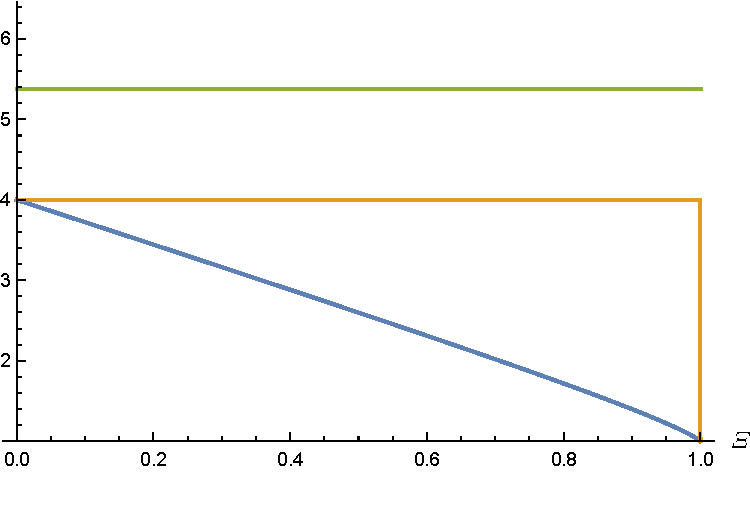
\includegraphics[scale=0.75]{convexity-bound}
\caption{Blue: the base of the exponential bound (\ref{convexityBound}) as a function of the
proportion of extreme points $\gX$. Yellow: the base of the pre-existing bound. We have a $4^n$
bound from the Sharir-Welzl theorem on matchings across a line, and for $\gh=1$ the bound becomes
subexponential---and is tight, and is $1$. Green: the bound (\ref{boundOnLeftRightPerfectMatchings})
on all of $\gn_{\pointset P}$ for comparison.\label{figConvexityBound}}
\end{figure}
\sectionorchapter{Three changes of bracket direction}
\label{sectionThreeChanges}
\begin{sloppypar}
We now consider perfect matchings consistent with bracket expressions which have three
changes of bracket directions\idest bracket expressions of the form
$\langle^a\rangle^b\langle^c\rangle^d$,
$a$ opening brackets, $b$ closing brackets, $c$ opening brackets, $d$ closing brackets, where
$a-b=d-c\geq 0$ and $a+b+c+d\DefinitionOf n$.
\end{sloppypar}

In term of points, this means that four sets can be separated by vertical lines, from left
to right, $a$ left-points forming the set $\pointset A$, $b$ right-points forming $\pointset B$,
$d$ left-points
forming $\pointset D$, and $c$ right-points forming $\pointset C$.
We pick a vertical line separating $\pointset A$ and $\pointset B$ and call it $V$, and we pick
a vertical line separating $\pointset C$ and $\pointset D$ and call it $W$,
see figure~\ref{figCFPMklqp}.

Given a crossing-free perfect matching on those points, numbering from top to bottom the
intersections between $V$ and edges incident to the points in $\pointset A$,
we get a crossing-free left-alignment $\ga$ of $\pointset A$ on $V$. $a-b$ of the $a$ edges
intersecting $V$
are incident to points in $\pointset D$; the other $b$ are incident to points in $\pointset B$.
Numbering those $b$ edges yields a crossing-free right-alignment $\gb$ of $\pointset B$ on $V$.

Similarly on the right side, we get a crossing-free right-alignment of $\gd$ of $\pointset D$ on $W$,
and numbering the subset of edges joining $\pointset C$ and $\pointset D$, we get a
left-alignment $\gg$ of $\pointset C$ on $W$.
\begin{figure}[!ht]
\centering
\begin{tikzpicture}[scale=0.5]
\tikzstyle{dot}=[draw,shape=circle,fill=black,scale=0.25]
\node[dot] at (-9,1.9) (k1) {};
\node[dot] at (-8,1) (k2) {};
\node[dot] at (-7,4) (k3) {};
\node[dot] at (-6,3) (k4) {};
\node[dot] at (-5,0) (k5) {};

\node[dot] at (-3.5,1.5) (l1) {};
\node[dot] at (-2.5,0.5) (l2) {};
\node[dot] at (-1.5,2.5) (l3) {};
\node[dot] at (-0.5,3) (l4) {};

\node[dot] at (0.5,3.7) (p1) {};
\node[dot] at (1.5,0) (p2) {};
\node[dot] at (2.5,1) (p3) {};
\node[dot] at (3.5,2.8) (p4) {};

\node[dot] at (5,2.5) (q1) {};
\node[dot] at (6,0.5) (q2) {};
\node[dot] at (7,3.5) (q3) {};
\node[dot] at (8,1.5) (q4) {};
\node[dot] at (9,2.1) (q5) {};

\draw[very thick, name path=left line] (-4.25,5) -- (-4.25,-1);
\draw[very thick, name path=right line] (4.25,5) -- (4.25,-1);

\draw[gray, name path=edge] (k1) -- (q5);
\draw[->,thick,name intersections={of=edge and left line, by=align}] (k1) -- (align);
\draw[->,thick,name intersections={of=edge and right line, by=align}] (q5) -- (align);


\draw[gray, name path=edge] (k3) -- (l4);
\draw[->,thick,name intersections={of=edge and left line, by=align}] (k3) -- (align);
\draw[->,thick,name intersections={of=edge and left line, by=align}] (l4) -- (align);

\draw[gray, name path=edge] (k2) -- (l1);
\draw[->,thick,name intersections={of=edge and left line, by=align}] (k2) -- (align);
\draw[->,thick,name intersections={of=edge and left line, by=align}] (l1) -- (align);

\draw[gray, name path=edge] (k4) -- (l3);
\draw[->,thick,name intersections={of=edge and left line, by=align}] (k4) -- (align);
\draw[->,thick,name intersections={of=edge and left line, by=align}] (l3) -- (align);

\draw[gray, name path=edge] (k5) -- (l2);
\draw[->,thick,name intersections={of=edge and left line, by=align}] (k5) -- (align);
\draw[->,thick,name intersections={of=edge and left line, by=align}] (l2) -- (align);


\draw[gray, name path=edge] (q1) -- (p4);
\draw[->,thick,name intersections={of=edge and right line, by=align}] (q1) -- (align);
\draw[->,thick,name intersections={of=edge and right line, by=align}] (p4) -- (align);

\draw[gray, name path=edge] (q2) -- (p2);
\draw[->,thick,name intersections={of=edge and right line, by=align}] (q2) -- (align);
\draw[->,thick,name intersections={of=edge and right line, by=align}] (p2) -- (align);

\draw[gray, name path=edge] (q3) -- (p1);
\draw[->,thick,name intersections={of=edge and right line, by=align}] (q3) -- (align);
\draw[->,thick,name intersections={of=edge and right line, by=align}] (p1) -- (align);

\draw[gray, name path=edge] (q4) -- (p3);
\draw[->,thick,name intersections={of=edge and right line, by=align}] (q4) -- (align);
\draw[->,thick,name intersections={of=edge and right line, by=align}] (p3) -- (align);

\node at (-9,-1) {$\langle$};
\node at (-8,-1) {$\langle$};
\node at (-7,-1) {$\langle$};
\node at (-6,-1) {$\langle$};
\node at (-5,-1) {$\langle$};

\node at (-7,5) {$\pointset A$};

\node at (-3.5,-1) {$\rangle$};
\node at (-2.5,-1) {$\rangle$};
\node at (-1.5,-1) {$\rangle$};
\node at (-0.5,-1) {$\rangle$};

\node at (-2,5) {$\pointset B$};
\node at (2,5) {$\pointset C$};

\node at (0.5,-1) {$\langle$};
\node at (1.5,-1) {$\langle$};
\node at (2.5,-1) {$\langle$};
\node at (3.5,-1) {$\langle$};

\node at (7,5) {$\pointset D$};

\node at (5,-1) {$\rangle$};
\node at (6,-1) {$\rangle$};
\node at (7,-1) {$\rangle$};
\node at (8,-1) {$\rangle$};
\node at (9,-1) {$\rangle$};

\node at (-4.25,5.5) {$V$};
\node at (4.25,5.5) {$W$};

\node at (-5,4.5) {$\ga$};
\node at (-3.5,4.5) {$\gb$};
\node at (3.5,4.5) {$\gg$};
\node at (5,4.5) {$\gd$};
\end{tikzpicture}
\caption{Four crossing-free alignments.\label{figCFPMklqp}}
\end{figure}
Call $\pointset S$ the set of $a-b$ points of $\pointset A$ that are matched with points of
$\pointset D$, and call $\pointset T$ the set of $d-c$ points of $\pointset D$ that are matched to points of
$\pointset A$.

\marginfig[Blue: the base $4x_\gh$ of the exponential bound (\ref{binomialBound}) for
$\gn_{\pointset P}\of{\langle^a\rangle^b\langle^b\rangle^a}$ as a function of
$\gh=\frac{b}{a}$. Yellow: the base of the pre-existing bound. We have a $4^n$
bound from the Sharir-Welzl theorem on matchings across a line when $\gh=0$ or $\gh=1$, otherwise
the pre-existing bound is (\ref{boundOnLeftRightPerfectMatchings}).
The bound is better than existing results for small and large $\gh$, but not for all $\gh$.
\label{figBinomialBound}]{%
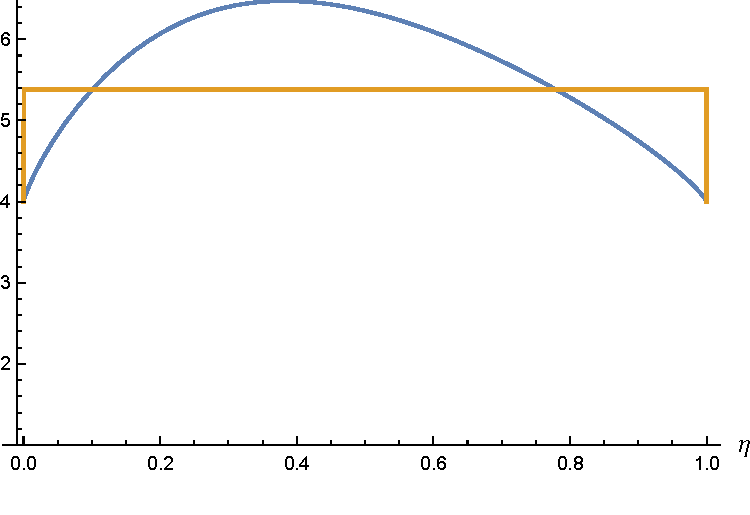
\includegraphics[scale=\minorplotsize]{binomial-bound}}
The matching is uniquely determined by $\ga$, $\gb$, the choice of
the subsets $\pointset S\Subset\pointset A$ and $\pointset T \Subset D$,
and by $\gb$ and $\gc$. This gives the following bound for the number of these matchings:
\begin{equation}
\gn_{\pointset P}\of{\langle^a\rangle^b\langle^c\rangle^d}
\leq \CatalanNumber a \binom a b \CatalanNumber b \CatalanNumber c \binom d c \CatalanNumber d\text.
\label{binomialBound}
\end{equation}
Asymptotically, the factor involving $a$ and $b$ is, for $b=\gh a$,\[
\CatalanNumber a \binom a b \CatalanNumber b
\preccurlyeq_{a+b}
4^{a+b} \binom a b
\preccurlyeq_{a+b}
4^{a+b}
\pa{
\underbrace{
\pa{\frac
  {\pa{1-\gh}^{1-\frac 1 \gh}}
  {\gh}}^{\frac{\gh}{\gh+1}}}_{x_\gh}}^{a+b}\text,
\]
uniformly in $\gh\in\intclos 01$. See figure~\ref{figBinomialBound} for a plot.
The base $x_\gh$ of the exponential bound for the binomial coefficient is
maximal\footnote{This can be shown by differentiating $x_\gh$.
One can alternatively study the sequence $\max_b \binom {m-b}{b}$, as in the
work of S.~M.~Tanny and M.~Zuker \cite{TannyZuker1974}.}
when $\gh = \frac{3-\sqrt{5}}{2}$, where it is $\GoldenRatio = \frac{1+\sqrt{5}}{2}$.
This gives the overall bound\[
\gn_{\pointset P}\of{\langle^a\rangle^b\langle^c\rangle^d}
\preccurlyeq_n
4^{a+b}
\GoldenRatio^{a+b}
4^{c+d}
\GoldenRatio^{c+d}
= \pa{4\GoldenRatio}^n
\approx 6.472^n
\]
uniformly in $a$, $b$, $c$, and $d$ such that $a+b+c+d=n$.
Note that this is worse than the existing $5.3793^n$ bound on $\gn_{\pointset P}\of{B}$ for an arbitrary
well-formed bracket expression $B$, see (\ref{boundOnLeftRightPerfectMatchings}).
\subsectionorsection{Improving upon the binomial bound}\label{ImprovingBinomial}
We can however improve upon that bound. Once $\ga$, $\gd$, $\pointset S$, and $\pointset T$
are fixed, the edges of the matching that cross both the left line
and the right line---let us call these \emph{long edges}---are determined.
As a result,
the strip $\gS$ between the vertical lines $V$ and $W$ is partitioned by the long edges in trapezoidal cells
$Z_1,\dotsc,Z_{a-b+1}$, numbered from top to bottom, where the first and last cells are
unbounded, see figure~\ref{figTrapezoids}.
\marginfig[The points of $\pointset S\Subset \pointset A$ and
$\pointset T\Subset \pointset D$ are shown in white.
The vertical lines $V$ and $W$ bound the strip $\gS$.
The long edges join $\pointset S$ and
$\pointset T$, partitioning the strip $\gS$ in cells $Z_i$.
The crossing-free right-alignments $\gb_i$ are shown.
Note that here $\pointset B_4$ is empty.
In this figure, $a=7$, $b=4$, $c=1$, and $d=4$.
\label{figTrapezoids}]{
\begin{tikzpicture}[scale=0.6]
\tikzstyle{dot}=[draw,shape=circle,fill=black,scale=0.5]
\tikzstyle{wdot}=[draw,shape=circle,fill=white,scale=0.5]

\draw[very thick, name path=V] (0,5) -- (0,-2);
\draw[very thick, name path=W] (4,5) -- (4,-2);


\node at (-1,5) {$\pointset A$};
\node at (5,5) {$\pointset D$};

\node at (0,5.5) {$V$};
\node at (4,5.5) {$W$};

\node at (2,-2) {$\gS$};

\node at (3,4.5) {$Z_1$};
\node at (3,2.5) {$Z_2$};
\node at (2.5,0.25) {$Z_3$};
\node at (1.5,-1) {$Z_4$};

\node[dot] at (-.5,4) (a1) {};
\node[wdot] at (-2,3.5) (a2) {};
\node[dot] at (-1.4,2.5) (a3) {};
\node[dot] at (-1.5,2) (a4) {};
\node[wdot] at (-1,1) (a5) {};
\node[dot] at (-1.3,0.5) (a6) {};
\node[wdot] at (-2.2,0) (a7) {};

\node[dot] at (2,4.2) (b1) {};
\node[dot] at (1.8,2.6) (b3) {};
\node[dot] at (2.2,1.8) (b4) {};
\node[dot] at (1.9,0.6) (b6) {};

\node[dot] at (3,0.3) (c) {};

\node[wdot] at (4.5,3.8) (d2) {};
\node[wdot] at (5,0.9) (d5) {};
\node[wdot] at (4.25,-.8) (d7) {};
\node[dot] at (5.25,0) (dc) {};

\draw (a2) -- (d2);
\draw (a5) -- (d5);
\draw (a7) -- (d7);

\draw[gray] (c) -- (dc);

\draw[gray, name path=edge] (a1) -- (b1);
\draw[->,thick,name intersections={of=edge and V, by=align}] (b1) -- (align);
\node[label={[font=\scriptsize,label distance=-3pt]above right:$1$}] at (align) {};
\draw[gray, name path=edge] (a3) -- (b3);
\draw[->,thick,name intersections={of=edge and V, by=align}] (b3) -- (align);
\node[label={[font=\scriptsize,label distance=-3pt]above right:$1$}] at (align) {};
\draw[gray, name path=edge] (a4) -- (b4);
\draw[->,thick,name intersections={of=edge and V, by=align}] (b4) -- (align);
\node[label={[font=\scriptsize,label distance=-3pt]below right:$2$}] at (align) {};
\draw[gray, name path=edge] (a6) -- (b6);
\draw[->,thick,name intersections={of=edge and V, by=align}] (b6) -- (align);
\node[label={[font=\scriptsize,label distance=-3pt]below right:$1$}] at (align) {};
\end{tikzpicture}}

We will consider the crossing-free right-alignment $\gb$; the same argument will hold for $\gg$.
Since $\pointset B$ lies within the strip $\gS$, it is partitioned in $a-b+1$ subsets
$\pointset B_i\DefineAs\pointset B \Intersection Z_i$.
Moreover, an edge $e_p$ emanating from a point $p\in\pointset B_i$ cannot cross the long edges,
and thus the portion $e_p\Intersection \gS$ of $e_p$ that lies within the strip $\gS$ is confined to the cell $Z_i$.

Let $\gb_i$ be the crossing-free right-alignment of $\pointset B_i$ on $V$ realized by
the segments $\setst{e_p\Intersection \gS}{p\in\pointset B_i}$.
Since the set of segments $\setst{e_p\Intersection \gS}{p\in\pointset B}$ realizes $\gb$,
$\gb$ is composed of the crossing-free right-alignments $\gb_i$. Formally, for
$p\in\pointset B_i$,
\[\gb\of p = \gb_i\of p + \sum{j=1}[i-1] \Cardinality{\pointset B_i}\text.\]
We now know that $\gb$ is determined by crossing-free alignments $\gb_i$ of point sets $\pointset B_i$.
In order to turn this into a bound, we need to know the sizes $\Cardinality{\pointset B_i}$ of these
point sets.
\marginfig[The edges crossing $V$. The points of $\pointset S$ are shown in white. The
crossing-free left-alignment $\ga$ of $\pointset A$ on $V$ is shown.
The elements of $S=\ga\of{\pointset S}$ are shown in red.
We have $\cells\of{[a]\setminus S}=\set{\set{1},\set{3,4},\set{6}}$.
Since $\pointset B_4$ is empty, there is no cell of ${[a]\setminus S}$
corresponding to it.\label{figCellsOnALine}]{
\begin{tikzpicture}[scale=0.6]
\tikzstyle{dot}=[draw,shape=circle,fill=black,scale=0.5]
\tikzstyle{wdot}=[draw,shape=circle,fill=white,scale=0.5]

\draw[very thick, name path=V] (0,5) -- (0,-2);
\path[name path=W] (3,5) -- (3,-2);

\node at (-2,5) {$\pointset A$};

\node at (0,5.5) {$V$};

\node at (3,4.5) {$\pointset B_1$};
\node at (3,2.5) {$\pointset B_2$};
\node at (3,0.25) {$\pointset B_3$};
\node at (3,-2) {$\pointset B_4 = \EmptySet$};

\node[dot] at (-.5,4.5) (a1) {};
\node[wdot] at (-2,3.5) (a2) {};
\node[dot] at (-1.4,2.5) (a3) {};
\node[dot] at (-1.5,2) (a4) {};
\node[wdot] at (-1,1) (a5) {};
\node[dot] at (-1.3,0) (a6) {};
\node[wdot] at (-2.2,-0.7) (a7) {};

\node[dot] at (2,4.7) (b1) {};
\node[dot] at (1.8,2.6) (b3) {};
\node[dot] at (2.2,1.8) (b4) {};
\node[dot] at (1.9,0.1) (b6) {};

\node at (4,3.8) (d2) {};
\node at (4,0.9) (d5) {};
\node at (4,-1.3) (d7) {};

\path[name path=long edge] (a2) -- (d2);
\draw[dashed,name intersections={of=long edge and W, by=far}] (d2) -- (far);
\draw (a2) -- (far);
\draw[->,thick,name intersections={of=long edge and V, by=align}] (a2) -- (align);
\node[label={[font=\scriptsize,label distance=-5pt]above left:$\color{red}2$}] at (align) {};

\path[name path=long edge] (a5) -- (d5);
\draw[dashed,name intersections={of=long edge and W, by=far}] (d5) -- (far);
\draw (a5) -- (far);
\draw[->,thick,name intersections={of=long edge and V, by=align}] (a5) -- (align);
\node[label={[font=\scriptsize,label distance=-5pt]below left:$\color{red}5$}] at (align) {};

\path[name path=long edge] (a7) -- (d7);
\draw[dashed,name intersections={of=long edge and W, by=far}] (d7) -- (far);
\draw (a7) -- (far);
\draw[->,thick,name intersections={of=long edge and V, by=align}] (a7) -- (align);
\node[label={[font=\scriptsize,label distance=-5pt]below left:$\color{red}7$}] at (align) {};

\draw[gray, name path=edge] (a1) -- (b1);
\draw[->,thick,name intersections={of=edge and V, by=align}] (a1) -- (align);
\node[label={[font=\scriptsize,label distance=-5pt]above left:$1$}] at (align) {};
\draw[gray, name path=edge] (a3) -- (b3);
\draw[->,thick,name intersections={of=edge and V, by=align}] (a3) -- (align);
\node[label={[font=\scriptsize,label distance=-5pt]above left:$3$}] at (align) {};
\draw[gray, name path=edge] (a4) -- (b4);
\draw[->,thick,name intersections={of=edge and V, by=align}] (a4) -- (align);
\node[label={[font=\scriptsize,label distance=-5pt]below left:$4$}] at (align) {};
\draw[gray, name path=edge] (a6) -- (b6);
\draw[->,thick,name intersections={of=edge and V, by=align}] (a6) -- (align);
\node[label={[font=\scriptsize,label distance=-5pt]below left:$6$}] at (align) {};
\end{tikzpicture}}

Let us look at the edges crossing $V$, numbered from top to bottom from $1$ to $a$, see
figure~\ref{figCellsOnALine}. Of these $a$ edges,
$a-b$ are long edges; they are the edges emanating from $\pointset S$. 
Their numbers are $S = \ga\of{\pointset S} \Subset [a]$.
The other edges are the ones that emanate from points of $\pointset B$.
Let $s_i$ be the $i$th element of $S$ in increasing order, thus $s_1=\min S$, and
$s_{\Cardinality S} = s_{a-b} = \max S$.

The numbering of the $a$ edges crossing $V$, from top to bottom, then starts with
the edges emanating from $\pointset B_1$, numbered $1$ through
$s_1-1$, the first long edge, numbered $s_1$, the edges emanating from
$\pointset B_2$, numbered $s_1+1$ through $s_2-1$, the second long edge,
numbered $s_2$, the edges emanating from $\pointset B_3$, numbered from $s_2+1$, \etc.
In other words, the numbers of the edges emanating from any nonempty $\pointset B_i$ forms
a maximal set of consecutive elements of $[a]\setminus S$. This motivates the following
definition.

\begin{sloppypar}
\begin{definition}[cells of a set of integers]
The \emph{cells} of $S'\Subset \N$, written $\cells\of{S'}$, is the set of maximal subsets of
consecutive elements $S'$.
\end{definition}
For instance, $\cells\of{\set{2,3,5,6,7,10,13,14}}=\set{\set{2,3},\set{5,6,7},\set{10},\set{13,14}}$.
\end{sloppypar}

Then, we can improve the $\binom a b \CatalanNumber b$ factor in the bound (in which the binomial comes from
the choice of $\pointset S$, and the Catalan number comes
from the choice of $\gb$), summing over the choices of $\pointset S$ (and thus of $S$ above).
The improved factor becomes\footnote{The name $\spc$ was chosen because we define this as
a Sum of Products of Catalan numbers.}\begin{equation}
\spc\of{a,b}\DefineAs
\sum{S\in\binom{[a]}{a-b}} \eggspacing{\quad} \prod{\gc\in\cells\of{[a] \setminus S}}\CatalanNumber {\Cardinality \gc} =
\sum{S'\in\binom{[a]}{b}} \eggspacing{\quad} \prod{\gc\in\cells\of{S'}}\CatalanNumber {\Cardinality \gc}\text,
\label{spcDefinition}
\end{equation}
and the overall bound becomes\begin{equation}
\gn_{\pointset P}\of{\langle^a\rangle^b\langle^c\rangle^d}\leq
\CatalanNumber a\spc\of{a, b}\spc\of{d, c}\CatalanNumber d\text.\label{bound-ck-spckl-spcpq-cp}
\end{equation}

\subsectionorsection{A recurrence}
In order to compute $\spc$ efficiently, and eventually, get its asymptotics, it is useful to get rid
of the $\cells$ function. We can express $\spc$ as a recurrence instead.
First, we note that $\spc\of{a,a} = \CatalanNumber a$: there is only one summand, $S'$ is the whole set, so
it has only one cell, namely $S'$ itself.
Otherwise, $a-b\geq 1$; in the sum over the $S$, consider the greatest element $j$ of $S$, which is at least
$a-b$, and split the sum over that,
\[\spc\of{a,b} = \sum{j=a-b}[a]\eggspacing{\quad\;}
\sum{\substack{S\in\binom{[a]}{a-b} \\ j=\max S}} \eggspacing{\quad}
\prod{\gc\in\cells\of{[a] \setminus S}}\CatalanNumber {\Cardinality \gc}\text.
\]
For fixed $j$, all summands (of the sum over $S$) will have a factor
with $\gc=\set{j+1,\dotsc,a}$, and thus a factor of
$\CatalanNumber {a-j}$. Factoring out this $\CatalanNumber {a-j}$, we get
\[\spc\of{a, b} = \sum{j=a-b}[a]
\CatalanNumber {a-j} \eggspacing{\;\;}
\sum{\substack{S\in\binom{[a]}{a-b} \\ j=\max S}} \eggspacing{\quad}
\prod{\substack{\gc\in\cells\of{[a] \setminus S} \\ \gc\neq\set{j+1,\dotsc,a}}}
    \CatalanNumber {\Cardinality \gc}\text.
\]
Now, note that choosing a subset $S$ of $[a]$ of size $a-b$ whose maximum is $j$ is equivalent to choosing
a subset $\tilde{S}$ of $[j-1]$ of size $a-b - 1$, where $S=\tilde{S}\Union\set{j}$.
Moreover, the cells of $[a]\setminus S$ other
than $\set{j+1,\dotsc,a}$ are exactly the cells of $[j-1]\setminus \tilde{S}$, thus
\[\spc\of{a,b} = \sum{j=a-b}[a]
\CatalanNumber {a-j} \eggspacing{\;\;}
\sum{\tilde{S}\in\binom{[j-1]}{a-b - 1}} \eggspacing{\quad\;}
\prod{\gc\in\cells\of{[j-1]\setminus \tilde{S}}}
    \CatalanNumber {\Cardinality \gc}\text.
\]
By definition of $\spc$, this means
\[\spc\of{a,b} = \sum{j=a-b}[a]
\CatalanNumber {a-j}
\spc\of{j-1,b+j-a}\text.
\]
Rewriting this as a sum over $i\DefineAs a-j$, this gives us the following recurrence for $\spc$:
\begin{align}\spc\of{a,b} &= \sum{i=0}[b]
\CatalanNumber {i}
\spc\of{a-i-1,b-i} &\text{for $b<a$,} \label{spcRecurrence1}\\
\spc\of{a,a} &= \CatalanNumber a \label{spckk}\text.
\end{align}\marginfig[The first few values of $\spc$; $a$ vertically from $0$ to $5$,
$b$ horizontally from $0$ to $a$. The values appearing in the $b+1$ summands of the
recurrence (\ref{spcRecurrence1}) with $a = 6$ and $b = 3$ are highlighted.]{
$\begin{array}{r r r r r r}
1 \\
{\color{red}1} & 1 \\
1 & {\color{red}2} &  2 \\
1 & 3 &  {\color{red}5} & 5 \\
1 & 4 &  9 & \tn{lastSummand}{\color{red}$14$} & 14 \\
1 & 5 & 14 & \tn{result}{$28$} & 42 & 42
\end{array}$
\tikz[remember picture,overlay]
    \path[->] (lastSummand.south) edge (result.north -| lastSummand.south);
}
We can use this recurrence directly to get a very slack bound on the asymptotics of (\ref{bound-ck-spckl-spcpq-cp}), see
appendix~\ref{appendixZetaBound}.
Since the recurrence allows for memoization, we can also compute $\spc$, and experimentally estimate its asymptotics, see
appendix~\ref{appendixExperimental}.
The $5^n$ bound that we can conjecture from these numerical calculations is much better than what we get by attempting to bound
this recurrence, so this motivates looking for a better one, to ultimately solve $\spc$.
\subsectionorsection{A better recurrence, and a solution}
We can now turn this recurrence into a simpler and better-known one, namely
\begin{align}
\spc\of{a,b} &= \spc\of{a-1, b} + \spc\of{a,b-1} & \text{for $a\geq 1$, $0\leq b \leq a$,}\label{spc-catalan-triangle}\\
\spc\of{a,b} &= 0 & \text{for $b < 0$ or $b > a$,}\label{degeneratespc}\\
\spc\of{0,0} &= 1 \label{spc00}\text.
\end{align}
Since $\spc$ has not been formally defined for negative arguments, we extend the definition
with $\spc\of{a,b}=0$ for $b<0$; this is consistent with original the definition, since it yields a sum over
subsets $S\Subset [a]$ bigger than $a$, and it yields an empty sum in the recurrence we just derived.
In addition to that, we also let $\spc\of{a,b} = 0$ when $b > a$. This takes care of (\ref{degeneratespc}).
Moreover, we know that $\spc\of{0,0}=\CatalanNumber 0=1$. There thus remains to prove (\ref{spc-catalan-triangle}).
We will do so first for $b=a$, then for $b=a-1$, and finally for the $0\leq b < a-1$.

Note that we have\begin{align}
\spc\of{b, b-1}
= \sum{i=0}[b-1]\CatalanNumber {i}\spc\of{b-i-1,b-i-1} 
= \sum{i=0}[b-1]\CatalanNumber {i}\CatalanNumber {b-i-1}
= \CatalanNumber {b}\text,\label{spckkminusone}
\end{align}
and thus, for $a=b > 0$,
\begin{equation}
\spc\of{a,b} = \CatalanNumber b = 0 + \CatalanNumber b = \spc\of{a-1, b} + \spc\of{a, b-1}.
\end{equation}
Further, for $a - 1 = b$, we get
\begin{align}
\spc\of{a,b}
&= \sum{i=0}[b]\CatalanNumber {i}\CatalanNumber {b-i} =
\CatalanNumber b + \sum{i=0}[b-1]\CatalanNumber{i}\CatalanNumber {b-i} \nonumber\\
\intertext{applying (\ref{spckk}) on the left and (\ref{spckkminusone}) on the right,}
&= \spc\of{a-1, b} + \sum{i=0}[b-1]\CatalanNumber {i}\spc\of{b-i,b-i-1} \nonumber\\
&= \spc\of{a-1, b} + \sum{i=0}[b-1]\CatalanNumber {i}\spc\of{a-i-1,b-i-1} \nonumber\\
&= \spc\of{a-1, b} + \spc\of{a,b-1}\text.
\end{align}

Now let $a - 1 > b \geq 0$.
Assume $\spc\of{a',b'}=\spc\of{a'-1,b'}+\spc\of{a',b'-1}$ for $0\leq b'<a'<a$.
Then we can apply this assumption to the summands of $\spc\of{a,b}$:
\begin{align}
\spc\of{a,b} &= \sum{i=0}[b]
\CatalanNumber {i}
\spc\of{a-i-1,b-i} \nonumber \\
&= \sum{i=0}[b]
\CatalanNumber {i}
\pa{\spc\of{a-i-2,b-i}+\spc\of{a-i-1,b-i-1}} \nonumber \\
&= \sum{i=0}[b]
\CatalanNumber {i}\spc\of{a-i-2,b-i}
+\sum{i=0}[b]\CatalanNumber {i}\spc\of{a-i-1,b-i-1} \nonumber \\
&= \sum{i=0}[b]
\CatalanNumber {i}\spc\of{(a-1)-i-1,b-i}
+\sum{i=0}[b-1]\CatalanNumber {i}\spc\of{a-i-1,(b-1)-i} \nonumber \\&\phantom{=}\eggspacing{\qquad} +
\underbrace{\CatalanNumber {b}\spc\of{a-b-1,-1}}_{=0}\text,
\nonumber \\
\intertext{so, by (\ref{spcRecurrence1}),}
&= \spc\of{a-1, b} + \spc\of{a,b-1}\text.
\end{align}
This completes the proof of (\ref{spc-catalan-triangle}).
\marginfig[The recurrence (\ref{spc-catalan-triangle}).]{
$\begin{array}{r r r r r r}
1 \\
1 & 1 \\
1 & 2 &  2 \\
1 & 3 &  5 & 5 \\
1 & 4 &  9 & \tn{summandAbove}{$14$} & 14 \\
1 & 5 & \tn{summandLeft}{$14$} & \tn{result}{$28$} & 42 & 42
\end{array}$
\tikz[remember picture,overlay]
    \path[->] (summandAbove.south) edge (result.north -| summandAbove.south)
              (summandLeft) edge (result);
}

The recurrence we just proved defines a triangle of numbers sometimes known as
the Catalan triangle\footnote{This triangle first appears as an example in a book by Arbogast in 1800 \cite{Arbogast1800}.
It features prominently in the previously-mentioned work of Errera \cite{Errera1931}, where it is
attributed to Delannoy, who defined it in 1889 \cite{Delannoy1889} as the number of paths by which a
rook can reach a square on a
triangular chessboard by going only down and right. The association with Catalan's name seems to come from a
1976 paper by Shapiro \cite{Shapiro1976}, where a definition similar to Delannoy's is independently given.
In that paper, the name is justified by (\ref{spckk}).}, and its solution is known, namely
\begin{equation}
\spc\of{a,b} = \frac
{\Factorial{\pa{a+b}} \pa{a-b+1}}
{\Factorial b \Factorial{\pa{a+1}}}
= \frac{a-b+1}{a+1} \binom{a+b}{a}\label{spc-solution}
\text,
\end{equation}
as shown by L.~F.~A.~Arbogast in 1800 \cite[p.~214--217]{Arbogast1800}.
\subsubsectionorsubsection{A combinatorial interpretation of \texorpdfstring{$\spc$}{spc}}
The Catalan triangle counts well-formed prefixes;
specifically, $\spc\of{a,b}$ is the number of well-formed prefixes with $a$ opening brackets
and $b$ closing brackets. This can in fact be seen from
all the definitions of $\spc$ above, thus providing a more combinatorial solution, as we will now see.

In the original definition (\ref{spcDefinition}) of $\spc$, the sum is over the choices for the positions of the
$a-b$ unmatched opening brackets; between those, well-formed bracket expressions (counted by Catalan numbers) are
inserted.

The first recurrence (\ref{spcRecurrence1}) corresponds to the following grammatical
definition\footnote{This grammar requires infinite look-ahead to parse, but doing a first pass to mark the
unmatched opening brackets resolves that.} of well-formed
prefixes, where again wfbe denotes a well-formed bracket expression:
\begin{align*}
\text{wfprefix} \Produces
& \text{wfbe} \langle \text{wfprefix} \\
\mid\: & \text{wfbe}.
\end{align*}
In this case the sum ranges over the length of the well-formed bracket expression preceding the first unmatched bracket.

Finally, (\ref{spc-catalan-triangle}) reflects the fact that a well-formed prefix with $a$ opening brackets
and $b$ closing brackets either ends with an opening bracket (preceded by a well-formed prefix with $a-1$ opening
and $b$ closing brackets), or with a closing bracket (preceded by a well-formed prefix with $a$ opening
and $b-1$ closing brackets).
\subsubsectionorsubsection{Tying up some loose ends}
\label{tyingLooseEnds}
We now solve the recurrence $\gcp$ defined in \sectionorchapterword~\ref{sectionHighlyConvex} by a combinatorial argument.
Recall that $\gcp$ is defined by
\begin{align*}
\gcp_{k,\gD}&\DefineAs\max_{\gD_1+\gD_2=\gD-1}\sum{i=\gD_1}[k-\gD_2-1]\gcp_{i,\gD_1}\gcp_{k-i-1,\gD_2}\text,\\
\gcp_{k,0}&\DefineAs\gcp_{k,1}\text{ for $k>0$, and}\\
\gcp_{k,k}&\DefineAs1\text.
\end{align*}
We will show that $\gcp\of{k,\gD}$ is the number of well-formed prefixes with $k$ opening brackets of which $\gD$
are unmatched, thus that $\gcp\of{k,\gD}=\spc\of{k,k-\gD}$.

Let $\gw_{k,\gD}\DefineAs\spc\of{k,k-\gD}$ be the number of well-formed prefixes with $k$ opening brackets of which $\gD$
are unmatched.
We have $\gw_{k,k}=1$, since the only such prefix is $\langle^k$.

Consider $\gw_{k,0}$ where $k>0$\idest the number of well-formed bracket expressions of length $k$. Note that any
nonempty well-formed bracket expression can be turned into a well-formed prefix with one unmatched opening bracket
by removing the final closing bracket, and that adding a closing bracket to a well-formed prefix with
one unmatched opening bracket yields a well-formed bracket expression. These operations are the inverse of each other,
thus they are bijections, so $\gw_{k,0}=\gw_{k,1}$.

Finally, we look at the sum. For any nonnegative $\gD_1$ and $\gD_2$ such that $\gD_1+\gD_2=\gD-1$,\[
\sum{i=\gD_1}[k-\gD_2-1]\gw_{i,\gD_1}\gw_{k-i-1,\gD_2}
\]
counts the number of ways of constructing a bracket expression with $k$ opening brackets of which $\gD$ are unmatched
by chaining
\begin{enumerate}
\item a prefix containing the first $\gD_1$ unmatched opening brackets;
\item an opening bracket, which will be unmatched;
\item a prefix containing the last $\gD_2$ unmatched opening brackets.
\end{enumerate}
Thus, for any nonnegative $\gD_1$ and $\gD_2$ such that $\gD_1+\gD_2=\gD-1$,\[
\gw_{k,\gD}=\sum{i=\gD_1}[k-\gD_2-1]\gw_{i,\gD_1}\gw_{k-i-1,\gD_2}\text.
\]
In particular,\[
\gw_{k,\gD}=\max_{\gD_1+\gD_2=\gD-1}\sum{i=\gD_1}[k-\gD_2-1]\gw_{i,\gD_1}\gw_{k-i-1,\gD_2}\text.
\]
It follows that $\gw=\gcp$; this completes the proof.
Substituting (\ref{spc-solution}), we get\begin{equation}
\gcp_{k,\gD}=\frac{\gD+1}{k+1}\binom{2k-\gD}{k}\text.
\end{equation}
\subsectionorsection{Asymptotics}
We can now use the expression (\ref{spc-solution}) for $\spc$ to study the properties of the bound
(\ref{bound-ck-spckl-spcpq-cp}).
First, we note that in the extreme case where $b=c=0$, so that the problem is that of matchings across
a line, the bound becomes ${\CatalanNumber a}^2$\idest we get exactly the Sharir--Welzl bound. When $a=b$ and
$c=d$, so that the bracket expression being considered is $\langle^a\rangle^a\langle^d\rangle^d$,
by (\ref{spckk}), we get a bound of ${\CatalanNumber a}^2{\CatalanNumber b}^2$. This is the bound that
is obtained from matchings across a line by chaining well-formed bracket expressions.
For nondegenerate cases, we look at the asymptotics.

We are interested in the asymptotics as a function of the length $n = a+b+c+d$ of the bracket expression.
Since the bound is a product of two identical two-parameter factors, we study one of them,\[
\gj_{a,b}\DefineAs \CatalanNumber a\spc\of{a,b}\text,
\]
as a function of $m\DefineAs a+b$. Let $b = \gh a$, thus $0\leq \gh\leq 1$,
the above expression becomes \[
\gj_{\frac{m}{\gh+1}, \frac{m\gh}{\gh+1}}=
\CatalanNumber {\frac{m}{\gh + 1}} \binom{m}{\frac{m}{\gh + 1}} \frac{m-m\gh+\gh+1}{m+\gh+1}
\leq \CatalanNumber {\frac{m}{\gh + 1}} \binom{m}{\frac{m}{\gh + 1}}\text.
\]
Asymptotically, this yields\[
\gj_{\frac{m}{\gh+1}, \frac{m\gh}{\gh+1}}\preccurlyeq_m
4^{\frac{m}{\gh + 1}}
\pa{
  \frac
    {\pa{1-\frac{1}{\gh+1}}^{\frac{1}{\gh+1}-1}}
    {\pa{\frac{1}{\gh+1}}^{\frac{1}{\gh+1}}}}^{m}
= \pa{\underbrace{4^{\frac{1}{\gh + 1}} \frac{\gh+1}{\gh^{\frac{\gh}{\gh+1}}}}_{y_\gh}}^m
\]
uniformly in $\gh\in\intclos 0 1$. See figure~\ref{figSpcBound} for a plot.
\begin{figure}[htb!]
\centering
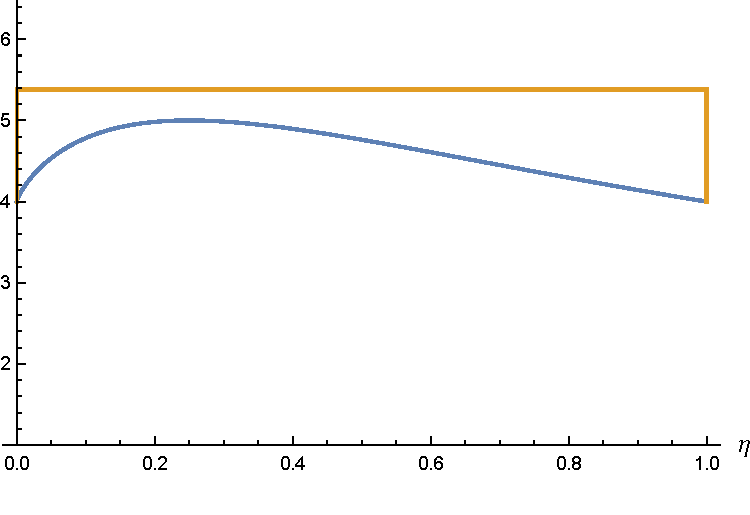
\includegraphics[scale=0.75]{spc-bound}
\caption{Blue: the base $y_\gh$ of the exponential bound (\ref{bound-ck-spckl-spcpq-cp}) for
$\gn_{\pointset P}\of{\langle^a\rangle^b\langle^b\rangle^a}$ as a function of
$\gh=\frac{b}{a}$. Yellow: the base of the pre-existing bound. We have a $4^n$
bound from the Sharir-Welzl theorem on matchings across a line when $\gh=0$ or $\gh=1$, otherwise
the pre-existing bound is (\ref{boundOnLeftRightPerfectMatchings}).\label{figSpcBound}}
\end{figure}

With some calculus, one can see that as $\gh$ ranges from $0$ to $1$,
the base $y_\gh$ of that exponential is maximal for
$\gh=\frac 1 4$, where its value is $5$.
We thus have the following asymptotic bound:\begin{equation}
\gn_{\pointset P}\of{\langle^a\rangle^b\langle^c\rangle^d}\leq
\CatalanNumber a\spc\of{a, b}\spc\of{d, c}\CatalanNumber d
\preccurlyeq_n
5^{a+b}5^{c+d} = 5^n
\end{equation}
uniformly in $a$, $b$, $c$, and $d$ such that $a+b+c+d=n$.
\sectionorchapter{Outlook}
As previously observed, uniform bounds on $\gn_{\pointset P}$ can be used to bound the number of
crossing-free perfect matchings, by summation over all bracket expressions. The bound derived in the previous
\sectionorchapterword only applies to a limited class of bracket expressions, and so it does not by itself
yield such an overall upper bound.

Moreover, while we used cones and conifers to improve the bound on the number of matchings across a
line, we did so only by looking at convexity properties, and we did not extend this reasoning
to the bracket expressions considered in \sectionorchapterword~\ref{sectionThreeChanges}.

We conclude this work by outlining a way in which the bound from \sectionorchapterword~\ref{sectionThreeChanges}
may be extended to arbitrary bracket expressions, and by discussing how conifers can be used to further
refine bounds regardless of the number of extreme points.

Recall that $\spc\of{a, b}$ counts the choices of ordering of the long edges crossing the strip $\gS$ on the left side of
that strip, together with (an upper bound on) right-alignments of the
right-points in the cells of that strip separated by the long edges.
Looking at an arbitrary well-formed bracket expression, we can separate it into\begin{enumerate}
\item a sequence of opening brackets $\langle^a$;
\item a sequence of expressions of the form $\rangle^{b_i}\langle^{c_i}$;
\item a sequence of closing brackets $\rangle^d$.
\end{enumerate}
The points $\pointset B_i$ and $\pointset C_i$ corresponding to the $\rangle^{b_i}\langle^{c_i}$ lie
within vertical strips $\gS_i$, and an
argument similar to section~\ref{ImprovingBinomial} can be made as follows.

Working from left to right, we pick a crossing-free right-alignment of the points $\pointset A$ corresponding
to $\langle^a$. Then, looking at a strip $\gS_i$, where the yet-unmatched points to the left of $\gS_i$ reach
its left side in a known vertical order, we choose which ones will cross the strip. This determines the size of
the sets $\pointset B_{ij} \Subset \pointset B_i$ of right-points within $\gS_i$ that are separated
by strip-crossing edges. Since the points from which the strip-crossing edges emanate are known,
the sizes determine the sets, since, as in section~\ref{MatchingsAcrossALine}, rotating an edge clockwise around its
left endpoint only adds to the set of points above it.
We then pick crossing-free right-alignments of the $\pointset B_{ij}$.
On the right side of the $\gS_i$, we pick the vertical indices of the
strip-crossing edges, and this determines the sizes, of the sets $\pointset C_{ij}\Subset \pointset C_i$
of left-points in $\gS_i$ separated by strip-crossing edges, and thus the $\pointset C_{ij}$ themselves.
We pick crossing-free left-alignments of the $\pointset C_{ij}$, and move on to strip $\gS_{i+1}$.
When we finally reach the points $\pointset D$ corresponding to $\rangle^d$, we pick a crossing-free right
alignment of them.

This yields a bound of\[
\gn_{\pointset P}\of{\langle^a\rangle^{b_1}\langle^{c_1}\dotsb\rangle^{b_r}\langle^{c_r}\rangle^d} \leq
\CatalanNumber a \CatalanNumber d
\prod{i=1}[r]\spc\of{a+\gt\of{i},b_i}
             \spc\of{a+\gt\of{i}-b_i,c_i}\text,\]
where $\gt\of{i}\DefineAs\sum{j=1}[i-1]\pa{c_j-b_j}$.
This bound is super-exponential: when $b_i=c_i=1$ for all $i$, we get
\[
\gn_{\pointset P}\of{\langle^a\rangle\langle\dotsb\rangle\langle\rangle^a}
\leq {\CatalanNumber a}^2 \spc\of{a, 1}^{2r}={\CatalanNumber a}^2 a^{2r}\text.\]
It may however be possible
to improve it with overcounting analyses similar to the one we suggest below.

Let us come back to crossing-free perfect matchings across a line. We have, based on conifers,\[
\gn_{\pointset P}\of{\langle^k\rangle^k}\leq \CatalanNumber k \CatalanNumber k
= \pa{\sum{i=0}[k-1]\CatalanNumber i \CatalanNumber {k-i-1}}
   \pa{\sum{j=0}[k-1]\CatalanNumber j \CatalanNumber {k-j-1}}\text,
\]
where in the first sum $i$ corresponds to the choice of the left $\pointset L$-cone $\lcone {i+1}$,
and in the second sum $j$ corresponds to the choice of the right $\pointset R$-cone $\rcone {j+1}$.
When expanding the product of these sums, the terms with $i=j$ count crossing-free perfect matchings
where the leftmost point is matched to the rightmost point. However, recall that to avoid overcounting,
a point must be matched within its cone. Since there is a single left-cone of $\pointset L$ that contains the
rightmost point, and a single right-cone of $\pointset R$ that contains the leftmost point, all but at most one
of the terms with $i=j$ are overcounted. We then get the bound\[
\gn_{\pointset P}\of{\langle^k\rangle^k}\leq
\max_{i\in\set{0,\dotsc,k-1}} \pa{\CatalanNumber i \CatalanNumber {k-i-1}}^2
+ \sum{i=0}[k-1]\sum{\substack{j=0\\ j\neq i}}[k-1] \CatalanNumber i \CatalanNumber {k-i-1}
                                                   \CatalanNumber j \CatalanNumber {k-j-1}\text.\]
It may then be possible to extend this reasoning to the rest of the conifers to get an asymptotic improvement.
\subsectionorsection*{Acknowledgements}
I would like to thank Emo~Welzl and Manuel~Wettstein for providing me with the opportunity to work on this subject, and for
their supervision and their numerous suggestions. In particular, Emo~Welzl suggested that I look for a bound dependent on
the number of extreme points, when I had used the reasoning of \sectionorchapterword~\ref{sectionHighlyConvex} only to
get a constant-factor improvement based on the fact that there are at least three extreme points, and Manuel~Wettstein
mentioned the combinatorial interpretation of $\spc$, without which solving $\gcp_{k,\gD}$ would have been far
more difficult.

Moreover, I thank Pascal~Leroy for jokingly suggesting the word ``conifer'', which turned out to be more appropriate than expected,
and, of course, I thank the \emph{On-Line Encyclopedia of Integer Sequences}, and \emph{Mathematica}.

